\INEchaptercarta{Nacimientos: características escolares de los padres}{}

\cajita{Nacimientos}{La tendencia en la cantidad de nacimientos ocurridos y registrados tiene una tendencia descendente desde el 2012, siendo para el 2014 un total de 386,195, cantidad menor en un 0.29\% respecto al año anterior.}{Nacimientos registrados}{República de Guatemala, serie histórica, en datos absolutos}{\ \\[0mm]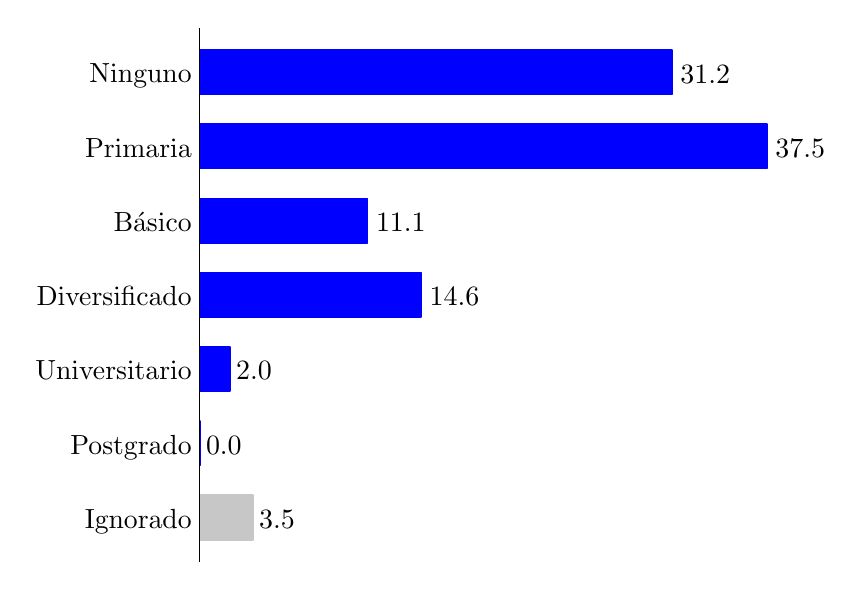
\begin{tikzpicture}[x=1pt,y=1pt]  % Created by tikzDevice version 0.7.0 on 2015-09-08 18:45:15
% !TEX encoding = UTF-8 Unicode
\definecolor[named]{fillColor}{rgb}{1.00,1.00,1.00}
\path[use as bounding box,fill=fillColor,fill opacity=0.00] (0,0) rectangle (289.08,198.74);
\begin{scope}
\path[clip] (  0.00,  0.00) rectangle (289.08,198.74);
\definecolor[named]{drawColor}{rgb}{1.00,1.00,1.00}

\path[draw=drawColor,line width= 0.6pt,line join=round,line cap=round] (  0.00,  0.00) rectangle (289.08,198.74);
\end{scope}
\begin{scope}
\path[clip] (  0.00,  0.00) rectangle (289.08,198.74);

\path[] ( 62.12,  5.69) rectangle (267.09,198.74);

\path[] ( 62.12, 21.78) --
	(267.09, 21.78);

\path[] ( 62.12, 48.59) --
	(267.09, 48.59);

\path[] ( 62.12, 75.40) --
	(267.09, 75.40);

\path[] ( 62.12,102.22) --
	(267.09,102.22);

\path[] ( 62.12,129.03) --
	(267.09,129.03);

\path[] ( 62.12,155.84) --
	(267.09,155.84);

\path[] ( 62.12,182.65) --
	(267.09,182.65);
\definecolor[named]{drawColor}{rgb}{0.78,0.78,0.78}
\definecolor[named]{fillColor}{rgb}{0.78,0.78,0.78}

\path[draw=drawColor,line width= 0.6pt,line join=round,fill=fillColor] ( 62.12, 13.73) rectangle ( 81.43, 29.82);
\definecolor[named]{drawColor}{rgb}{0.00,0.00,1.00}
\definecolor[named]{fillColor}{rgb}{0.00,0.00,1.00}

\path[draw=drawColor,line width= 0.6pt,line join=round,fill=fillColor] ( 62.12, 40.55) rectangle ( 62.21, 56.63);

\path[draw=drawColor,line width= 0.6pt,line join=round,fill=fillColor] ( 62.12, 67.36) rectangle ( 73.11, 83.45);

\path[draw=drawColor,line width= 0.6pt,line join=round,fill=fillColor] ( 62.12, 94.17) rectangle (142.17,110.26);

\path[draw=drawColor,line width= 0.6pt,line join=round,fill=fillColor] ( 62.12,120.99) rectangle (122.75,137.07);

\path[draw=drawColor,line width= 0.6pt,line join=round,fill=fillColor] ( 62.12,147.80) rectangle (267.09,163.89);

\path[draw=drawColor,line width= 0.6pt,line join=round,fill=fillColor] ( 62.12,174.61) rectangle (232.77,190.70);
\definecolor[named]{drawColor}{rgb}{0.00,0.00,0.00}
\definecolor[named]{fillColor}{rgb}{0.00,0.00,0.00}

\path[draw=drawColor,line width= 0.1pt,line join=round,fill=fillColor] ( 62.12,  5.69) -- ( 62.12,198.74);

\node[text=drawColor,anchor=base west,inner sep=0pt, outer sep=0pt, scale=  1.01] at ( 83.67, 17.82) {3.5};

\node[text=drawColor,anchor=base west,inner sep=0pt, outer sep=0pt, scale=  1.01] at ( 64.44, 44.63) {0.0};

\node[text=drawColor,anchor=base west,inner sep=0pt, outer sep=0pt, scale=  1.01] at ( 75.34, 71.45) {2.0};

\node[text=drawColor,anchor=base west,inner sep=0pt, outer sep=0pt, scale=  1.01] at (145.29, 98.26) {14.6};

\node[text=drawColor,anchor=base west,inner sep=0pt, outer sep=0pt, scale=  1.01] at (125.87,125.07) {11.1};

\node[text=drawColor,anchor=base west,inner sep=0pt, outer sep=0pt, scale=  1.01] at (270.20,151.89) {37.5};

\node[text=drawColor,anchor=base west,inner sep=0pt, outer sep=0pt, scale=  1.01] at (235.89,178.70) {31.2};
\end{scope}
\begin{scope}
\path[clip] (  0.00,  0.00) rectangle (289.08,198.74);

\path[] ( 62.12,  5.69) --
	( 62.12,198.74);
\end{scope}
\begin{scope}
\path[clip] (  0.00,  0.00) rectangle (289.08,198.74);
\definecolor[named]{drawColor}{rgb}{0.00,0.00,0.00}

\node[text=drawColor,anchor=base east,inner sep=0pt, outer sep=0pt, scale=  1.00] at ( 59.27, 17.87) {Ignorado};

\node[text=drawColor,anchor=base east,inner sep=0pt, outer sep=0pt, scale=  1.00] at ( 59.27, 44.68) {Postgrado};

\node[text=drawColor,anchor=base east,inner sep=0pt, outer sep=0pt, scale=  1.00] at ( 59.27, 71.50) {Universitario};

\node[text=drawColor,anchor=base east,inner sep=0pt, outer sep=0pt, scale=  1.00] at ( 59.27, 98.31) {Diversificado};

\node[text=drawColor,anchor=base east,inner sep=0pt, outer sep=0pt, scale=  1.00] at ( 59.27,125.12) {B\'asico};

\node[text=drawColor,anchor=base east,inner sep=0pt, outer sep=0pt, scale=  1.00] at ( 59.27,151.93) {Primaria};

\node[text=drawColor,anchor=base east,inner sep=0pt, outer sep=0pt, scale=  1.00] at ( 59.27,178.75) {Ninguno};
\end{scope}
\begin{scope}
\path[clip] (  0.00,  0.00) rectangle (289.08,198.74);

\path[] ( 59.27, 21.78) --
	( 63.54, 21.78);

\path[] ( 59.27, 48.59) --
	( 63.54, 48.59);

\path[] ( 59.27, 75.40) --
	( 63.54, 75.40);

\path[] ( 59.27,102.22) --
	( 63.54,102.22);

\path[] ( 59.27,129.03) --
	( 63.54,129.03);

\path[] ( 59.27,155.84) --
	( 63.54,155.84);

\path[] ( 59.27,182.65) --
	( 63.54,182.65);
\end{scope}
\begin{scope}
\path[clip] (  0.00,  0.00) rectangle (289.08,198.74);

\path[] ( 62.12,  5.69) --
	(267.09,  5.69);
\end{scope}
  \end{tikzpicture}}{Instituto Nacional de Estadística, de las Estadísticas Vitales 2014}

\cajita{Escolaridad de la madre}{Para el 2014, del total de nacimientos, el 37.4\% fueron en madres que tenían algún grado de educación primaria, el 17.5\% algún grado de educación media y el 2.0\% formación universitaria.
	
	En el 30.3\% de los casos, las madres no tenían ningún nivel de escolaridad.}{Distribución porcentual de los nacimientos según nivel de educación de las madres}{República de Guatemala, 2014, en porcentaje}{\ \\[0mm]\begin{tikzpicture}[x=1pt,y=1pt]  % Created by tikzDevice version 0.7.0 on 2015-08-28 14:35:13
% !TEX encoding = UTF-8 Unicode
\definecolor[named]{fillColor}{rgb}{1.00,1.00,1.00}
\path[use as bounding box,fill=fillColor,fill opacity=0.00] (0,0) rectangle (289.08,198.74);
\begin{scope}
\path[clip] (  0.00,  0.00) rectangle (289.08,198.74);
\definecolor[named]{drawColor}{rgb}{1.00,1.00,1.00}

\path[draw=drawColor,line width= 0.6pt,line join=round,line cap=round] (  0.00,  0.00) rectangle (289.08,198.74);
\end{scope}
\begin{scope}
\path[clip] (  0.00,  0.00) rectangle (289.08,198.74);

\path[] (  1.64, 17.78) rectangle (280.54,191.48);

\path[] (  1.64, 46.56) --
	(280.54, 46.56);

\path[] (  1.64, 88.34) --
	(280.54, 88.34);

\path[] (  1.64,130.11) --
	(280.54,130.11);

\path[] (  1.64,171.89) --
	(280.54,171.89);

\path[] (  1.64, 25.67) --
	(280.54, 25.67);

\path[] (  1.64, 67.45) --
	(280.54, 67.45);

\path[] (  1.64,109.22) --
	(280.54,109.22);

\path[] (  1.64,151.00) --
	(280.54,151.00);

\path[] ( 41.49, 17.78) --
	( 41.49,191.48);

\path[] (107.89, 17.78) --
	(107.89,191.48);

\path[] (174.30, 17.78) --
	(174.30,191.48);

\path[] (240.70, 17.78) --
	(240.70,191.48);
\definecolor[named]{drawColor}{rgb}{0.00,0.00,1.00}

\path[draw=drawColor,line width= 1.7pt,line join=round] ( 41.49,183.59) --
	(107.89,177.32) --
	(174.30,163.53) --
	(240.70,156.01);
\definecolor[named]{drawColor}{rgb}{0.00,0.00,0.00}

\node[text=drawColor,anchor=base,inner sep=0pt, outer sep=0pt, scale=  1.01] at ( 41.49,187.54) {37.8};

\node[text=drawColor,anchor=base west,inner sep=0pt, outer sep=0pt, scale=  1.01] at (107.89,181.28) {36.3};

\node[text=drawColor,anchor=base west,inner sep=0pt, outer sep=0pt, scale=  1.01] at (174.30,167.49) {33.0};

\node[text=drawColor,anchor=base,inner sep=0pt, outer sep=0pt, scale=  1.01] at (240.70,144.14) {31.2};
\definecolor[named]{fillColor}{rgb}{0.00,0.00,0.00}

\path[draw=drawColor,line width= 0.1pt,line join=round,fill=fillColor] (  1.64, 25.67) -- (280.54, 25.67);
\end{scope}
\begin{scope}
\path[clip] (  0.00,  0.00) rectangle (289.08,198.74);

\path[] (  1.64, 17.78) --
	(  1.64,191.48);
\end{scope}
\begin{scope}
\path[clip] (  0.00,  0.00) rectangle (289.08,198.74);

\path[] (  0.00, 25.67) --
	(  1.64, 25.67);

\path[] (  0.00, 67.45) --
	(  1.64, 67.45);

\path[] (  0.00,109.22) --
	(  1.64,109.22);

\path[] (  0.00,151.00) --
	(  1.64,151.00);
\end{scope}
\begin{scope}
\path[clip] (  0.00,  0.00) rectangle (289.08,198.74);

\path[] (  1.64, 17.78) --
	(280.54, 17.78);
\end{scope}
\begin{scope}
\path[clip] (  0.00,  0.00) rectangle (289.08,198.74);

\path[] ( 41.49, 13.51) --
	( 41.49, 17.78);

\path[] (107.89, 13.51) --
	(107.89, 17.78);

\path[] (174.30, 13.51) --
	(174.30, 17.78);

\path[] (240.70, 13.51) --
	(240.70, 17.78);
\end{scope}
\begin{scope}
\path[clip] (  0.00,  0.00) rectangle (289.08,198.74);
\definecolor[named]{drawColor}{rgb}{0.00,0.00,0.00}

\node[text=drawColor,anchor=base,inner sep=0pt, outer sep=0pt, scale=  1.00] at ( 41.49,  2.85) {2010};

\node[text=drawColor,anchor=base,inner sep=0pt, outer sep=0pt, scale=  1.00] at (107.89,  2.85) {2011};

\node[text=drawColor,anchor=base,inner sep=0pt, outer sep=0pt, scale=  1.00] at (174.30,  2.85) {2012};

\node[text=drawColor,anchor=base,inner sep=0pt, outer sep=0pt, scale=  1.00] at (240.70,  2.85) {2014};
\end{scope}
  \end{tikzpicture}}{Instituto Nacional de Estadística, de las Estadísticas Vitales 2014}

\cajita{Madres sin escolaridad}{En cuanto a la tendencia en la proporción de nacimientos en madres sin ningún nivel de escolaridad, esta es descendente, de 37.8\% a 30.3\%, en el período mostrado, que en términos absolutos significa que disminuyó de 136,764 a 117,064 nacimientos.}{Proporción de nacimientos en madres sin escolaridad}{República de Guatemala, serie histórica, en porcentaje}{\ \\[0mm]\begin{tikzpicture}[x=1pt,y=1pt]  % Created by tikzDevice version 0.10.1 on 2016-02-29 14:38:42
% !TEX encoding = UTF-8 Unicode
\definecolor{fillColor}{RGB}{255,255,255}
\path[use as bounding box,fill=fillColor,fill opacity=0.00] (0,0) rectangle (289.08,198.74);
\begin{scope}
\path[clip] (  0.00,  0.00) rectangle (289.08,198.74);

\path[] (  0.00,  0.00) rectangle (289.08,198.74);
\end{scope}
\begin{scope}
\path[clip] (  0.00,  0.00) rectangle (289.08,198.74);

\path[] ( -0.52, 15.61) rectangle (280.54,191.48);

\path[] (  0.00, 44.75) --
	(280.54, 44.75);

\path[] (  0.00, 87.05) --
	(280.54, 87.05);

\path[] (  0.00,129.35) --
	(280.54,129.35);

\path[] (  0.00,171.65) --
	(280.54,171.65);

\path[] (  0.00, 23.61) --
	(280.54, 23.61);

\path[] (  0.00, 65.90) --
	(280.54, 65.90);

\path[] (  0.00,108.20) --
	(280.54,108.20);

\path[] (  0.00,150.50) --
	(280.54,150.50);

\path[] ( 31.91, 15.61) --
	( 31.91,191.48);

\path[] ( 85.96, 15.61) --
	( 85.96,191.48);

\path[] (140.01, 15.61) --
	(140.01,191.48);

\path[] (194.06, 15.61) --
	(194.06,191.48);

\path[] (248.11, 15.61) --
	(248.11,191.48);
\definecolor{drawColor}{RGB}{0,0,255}

\path[draw=drawColor,line width= 1.7pt,line join=round] ( 31.91,183.49) --
	( 85.96,177.14) --
	(140.01,163.19) --
	(194.06,155.57) --
	(248.11,151.82);
\definecolor{drawColor}{RGB}{0,0,0}

\node[text=drawColor,anchor=base,inner sep=0pt, outer sep=0pt, scale=  1.02] at ( 31.91,187.46) {37.8};

\node[text=drawColor,anchor=base west,inner sep=0pt, outer sep=0pt, scale=  1.02] at ( 85.96,181.12) {36.3};

\node[text=drawColor,anchor=base west,inner sep=0pt, outer sep=0pt, scale=  1.02] at (140.01,167.16) {33.0};

\node[text=drawColor,anchor=base west,inner sep=0pt, outer sep=0pt, scale=  1.02] at (194.06,159.54) {31.2};

\node[text=drawColor,anchor=base,inner sep=0pt, outer sep=0pt, scale=  1.02] at (248.11,139.90) {30.3};

\path[draw=drawColor,line width= 0.1pt,line join=round] (  0.00, 23.61) -- (280.54, 23.61);

\path[] ( -0.52, 15.61) rectangle (280.54,191.48);
\end{scope}
\begin{scope}
\path[clip] (  0.00,  0.00) rectangle (289.08,198.74);

\path[] (  0.00, 15.61) --
	(280.54, 15.61);
\end{scope}
\begin{scope}
\path[clip] (  0.00,  0.00) rectangle (289.08,198.74);

\path[] ( 31.91, 12.86) --
	( 31.91, 15.61);

\path[] ( 85.96, 12.86) --
	( 85.96, 15.61);

\path[] (140.01, 12.86) --
	(140.01, 15.61);

\path[] (194.06, 12.86) --
	(194.06, 15.61);

\path[] (248.11, 12.86) --
	(248.11, 15.61);
\end{scope}
\begin{scope}
\path[clip] (  0.00,  0.00) rectangle (289.08,198.74);
\definecolor{drawColor}{RGB}{0,0,0}

\node[text=drawColor,anchor=base,inner sep=0pt, outer sep=0pt, scale=  1.00] at ( 31.91,  2.85) {2010};

\node[text=drawColor,anchor=base,inner sep=0pt, outer sep=0pt, scale=  1.00] at ( 85.96,  2.85) {2011};

\node[text=drawColor,anchor=base,inner sep=0pt, outer sep=0pt, scale=  1.00] at (140.01,  2.85) {2012};

\node[text=drawColor,anchor=base,inner sep=0pt, outer sep=0pt, scale=  1.00] at (194.06,  2.85) {2013};

\node[text=drawColor,anchor=base,inner sep=0pt, outer sep=0pt, scale=  1.00] at (248.11,  2.85) {2014};
\end{scope}
  \end{tikzpicture}}{Instituto Nacional de Estadística, de las Estadísticas Vitales 2014}	

\cajita{Madres sin escolaridad por etnia}{Según el grupo étnico de la madre, del total de nacimientos en madres indígenas, el 42.8\% no tenía ningún nivel de escolaridad, mayor que la proporción nacional en casi 13 puntos porcentuales. 
	
	Por otro lado, en el grupo étnico ladino-mestizo esta proporción fue de 15.7\%.}{Proporción de nacimientos en madres sin escolaridad según grupo étnico}{República de Guatemala, serie histórica, en porcentaje}{\ \\[0mm]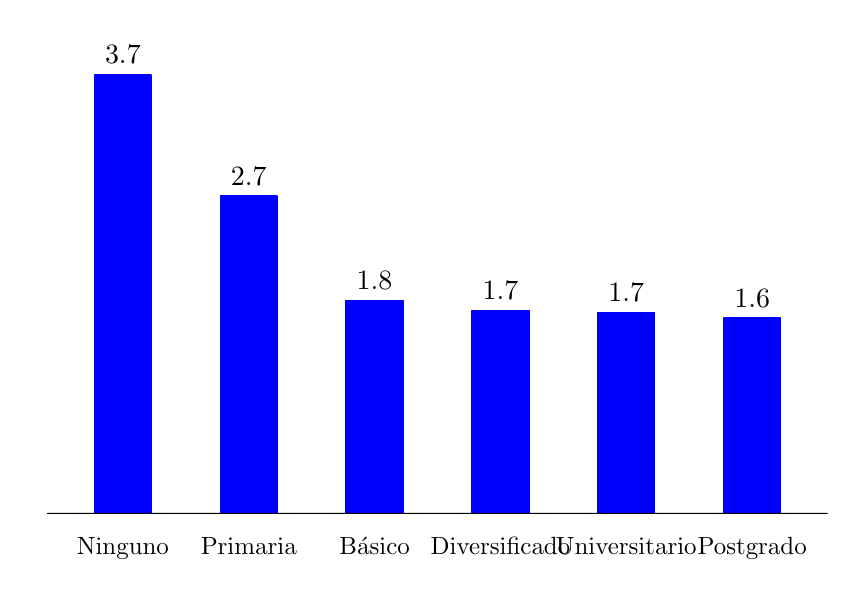
\begin{tikzpicture}[x=1pt,y=1pt]  % Created by tikzDevice version 0.7.0 on 2015-08-28 14:35:16
% !TEX encoding = UTF-8 Unicode
\definecolor[named]{fillColor}{rgb}{1.00,1.00,1.00}
\path[use as bounding box,fill=fillColor,fill opacity=0.00] (0,0) rectangle (289.08,198.74);
\begin{scope}
\path[clip] (  0.00,  0.00) rectangle (289.08,198.74);
\definecolor[named]{drawColor}{rgb}{1.00,1.00,1.00}

\path[draw=drawColor,line width= 0.6pt,line join=round,line cap=round] (  0.00,  0.00) rectangle (289.08,198.74);
\end{scope}
\begin{scope}
\path[clip] (  0.00,  0.00) rectangle (289.08,198.74);

\path[] (  7.11, 23.47) rectangle (289.08,181.67);

\path[] ( 34.40, 23.47) --
	( 34.40,181.67);

\path[] ( 79.88, 23.47) --
	( 79.88,181.67);

\path[] (125.36, 23.47) --
	(125.36,181.67);

\path[] (170.84, 23.47) --
	(170.84,181.67);

\path[] (216.31, 23.47) --
	(216.31,181.67);

\path[] (261.79, 23.47) --
	(261.79,181.67);
\definecolor[named]{drawColor}{rgb}{0.00,0.00,1.00}
\definecolor[named]{fillColor}{rgb}{0.00,0.00,1.00}

\path[draw=drawColor,line width= 0.6pt,line join=round,fill=fillColor] ( 24.17, 23.47) rectangle ( 44.63,181.67);

\path[draw=drawColor,line width= 0.6pt,line join=round,fill=fillColor] ( 69.65, 23.47) rectangle ( 90.11,137.82);

\path[draw=drawColor,line width= 0.6pt,line join=round,fill=fillColor] (115.12, 23.47) rectangle (135.59,100.14);

\path[draw=drawColor,line width= 0.6pt,line join=round,fill=fillColor] (160.60, 23.47) rectangle (181.07, 96.49);

\path[draw=drawColor,line width= 0.6pt,line join=round,fill=fillColor] (206.08, 23.47) rectangle (226.55, 95.78);

\path[draw=drawColor,line width= 0.6pt,line join=round,fill=fillColor] (251.56, 23.47) rectangle (272.03, 93.77);
\definecolor[named]{drawColor}{rgb}{0.00,0.00,0.00}
\definecolor[named]{fillColor}{rgb}{0.00,0.00,0.00}

\path[draw=drawColor,line width= 0.1pt,line join=round,fill=fillColor] (  7.11, 23.47) -- (289.08, 23.47);

\node[text=drawColor,anchor=base,inner sep=0pt, outer sep=0pt, scale=  1.01] at ( 34.40,185.63) {3.7};

\node[text=drawColor,anchor=base,inner sep=0pt, outer sep=0pt, scale=  1.01] at ( 79.88,141.77) {2.7};

\node[text=drawColor,anchor=base,inner sep=0pt, outer sep=0pt, scale=  1.01] at (125.36,104.10) {1.8};

\node[text=drawColor,anchor=base,inner sep=0pt, outer sep=0pt, scale=  1.01] at (170.84,100.44) {1.7};

\node[text=drawColor,anchor=base,inner sep=0pt, outer sep=0pt, scale=  1.01] at (216.31, 99.73) {1.7};

\node[text=drawColor,anchor=base,inner sep=0pt, outer sep=0pt, scale=  1.01] at (261.79, 97.73) {1.6};
\end{scope}
\begin{scope}
\path[clip] (  0.00,  0.00) rectangle (289.08,198.74);

\path[] (  7.11, 23.47) --
	(  7.11,181.67);
\end{scope}
\begin{scope}
\path[clip] (  0.00,  0.00) rectangle (289.08,198.74);

\path[] (  7.11, 23.47) --
	(289.08, 23.47);
\end{scope}
\begin{scope}
\path[clip] (  0.00,  0.00) rectangle (289.08,198.74);

\path[] ( 34.40, 19.20) --
	( 34.40, 23.47);

\path[] ( 79.88, 19.20) --
	( 79.88, 23.47);

\path[] (125.36, 19.20) --
	(125.36, 23.47);

\path[] (170.84, 19.20) --
	(170.84, 23.47);

\path[] (216.31, 19.20) --
	(216.31, 23.47);

\path[] (261.79, 19.20) --
	(261.79, 23.47);
\end{scope}
\begin{scope}
\path[clip] (  0.00,  0.00) rectangle (289.08,198.74);
\definecolor[named]{drawColor}{rgb}{0.00,0.00,0.00}

\node[text=drawColor,anchor=base,inner sep=0pt, outer sep=0pt, scale=  0.9] at ( 34.40,  8.54) {Ninguno};

\node[text=drawColor,anchor=base,inner sep=0pt, outer sep=0pt, scale=  0.9] at ( 79.88,  8.54) {Primaria};

\node[text=drawColor,anchor=base,inner sep=0pt, outer sep=0pt, scale=  0.9] at (125.36,  8.54) {B\'asico};

\node[text=drawColor,anchor=base,inner sep=0pt, outer sep=0pt, scale= 0.9] at (170.84,  8.54) {Diversificado};

\node[text=drawColor,anchor=base,inner sep=0pt, outer sep=0pt, scale=  0.9] at (216.31,  8.54) {Universitario};

\node[text=drawColor,anchor=base,inner sep=0pt, outer sep=0pt, scale=  0.9] at (261.79,  8.54) {Postgrado};
\end{scope}
  \end{tikzpicture}}{Instituto Nacional de Estadística, de las Estadísticas Vitales 2014}



\cajota{Madres sin escolaridad en los departamentos}{Para el 2014, a nivel departamental, se presentan las mayores proporciones de nacimientos en madres sin educación en la región VII: Quiché (51.6\%), región II: Alta Verapaz (48.6\%) y Baja Verapaz (40.1\%), región IV: Jalapa (43.0\%), región III: Chiquimula (41.9\%)
	
	 Los departamentos con menor porcentaje fueron Guatemala (12.0\%), El Progreso (15.8\%), Chimaltenango (16.3\%).}{Proporción de nacimientos en madres sin escolaridad }{Departamental, 2014, en porcentaje}{\includegraphics[width=52\cuadri]{graficas/vitales/Hoja5.pdf}}{Instituto Nacional de Estadística, de las Estadísticas Vitales 2014}




% % % % %Hoja21

\cajita{Edad de las madres}{En los nacimientos de 2014, el mayor edad mediana de las madres de acuerdo a su nivel de escolaridad fue en las madres con doctorado, el cual fue de 35 años. El menor se presenta en las madres con nivel de educación básica, el cual fue de 23.1 años.}{Edad promedio de las madres según escolaridad}{República de Guatemala, año 2014, en años}{\ \\[0mm]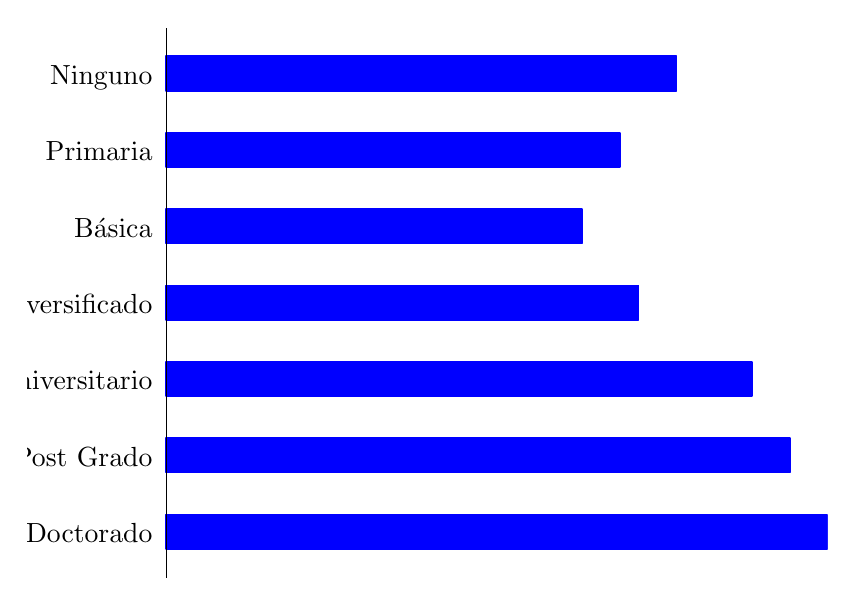
\begin{tikzpicture}[x=1pt,y=1pt]  % Created by tikzDevice version 0.10.1 on 2016-02-29 14:47:24
% !TEX encoding = UTF-8 Unicode
\definecolor{fillColor}{RGB}{255,255,255}
\path[use as bounding box,fill=fillColor,fill opacity=0.00] (0,0) rectangle (289.08,198.74);
\begin{scope}
\path[clip] (  0.00,  0.00) rectangle (289.08,198.74);

\path[] (  0.00,  0.00) rectangle (289.08,198.74);
\end{scope}
\begin{scope}
\path[clip] (  0.00,  0.00) rectangle (289.08,198.74);

\path[] ( 50.00,  0.00) rectangle (289.08,198.74);

\path[] ( 50.00, 16.56) --
	(289.08, 16.56);

\path[] ( 50.00, 44.16) --
	(289.08, 44.16);

\path[] ( 50.00, 71.77) --
	(289.08, 71.77);

\path[] ( 50.00, 99.37) --
	(289.08, 99.37);

\path[] ( 50.00,126.97) --
	(289.08,126.97);

\path[] ( 50.00,154.58) --
	(289.08,154.58);

\path[] ( 50.00,182.18) --
	(289.08,182.18);
\definecolor{drawColor}{RGB}{0,0,255}
\definecolor{fillColor}{RGB}{0,0,255}

\path[draw=drawColor,line width= 0.6pt,line join=round,fill=fillColor] ( 50.00, 10.35) rectangle (289.08, 22.77);

\path[draw=drawColor,line width= 0.6pt,line join=round,fill=fillColor] ( 50.00, 37.95) rectangle (275.42, 50.38);

\path[draw=drawColor,line width= 0.6pt,line join=round,fill=fillColor] ( 50.00, 65.56) rectangle (261.76, 77.98);

\path[draw=drawColor,line width= 0.6pt,line join=round,fill=fillColor] ( 50.00, 93.16) rectangle (220.77,105.58);

\path[draw=drawColor,line width= 0.6pt,line join=round,fill=fillColor] ( 50.00,120.76) rectangle (200.28,133.19);

\path[draw=drawColor,line width= 0.6pt,line join=round,fill=fillColor] ( 50.00,148.37) rectangle (213.94,160.79);

\path[draw=drawColor,line width= 0.6pt,line join=round,fill=fillColor] ( 50.00,175.97) rectangle (234.43,188.39);
\definecolor{drawColor}{RGB}{0,0,0}

\path[draw=drawColor,line width= 0.1pt,line join=round] ( 50.00,  0.00) -- ( 50.00,198.74);

\path[] ( 50.00,  0.00) rectangle (289.08,198.74);
\end{scope}
\begin{scope}
\path[clip] (  0.00,  0.00) rectangle (289.08,198.74);

\path[] ( 50.00,  0.00) --
	( 50.00,198.74);
\end{scope}
\begin{scope}
\path[clip] (  0.00,  0.00) rectangle (289.08,198.74);
\definecolor{drawColor}{RGB}{0,0,0}

\node[text=drawColor,anchor=base east,inner sep=0pt, outer sep=0pt, scale=  1.00] at ( 45.05, 12.65) {Doctorado};

\node[text=drawColor,anchor=base east,inner sep=0pt, outer sep=0pt, scale=  1.00] at ( 45.05, 40.26) {Post Grado};

\node[text=drawColor,anchor=base east,inner sep=0pt, outer sep=0pt, scale=  1.00] at ( 45.05, 67.86) {Universitario};

\node[text=drawColor,anchor=base east,inner sep=0pt, outer sep=0pt, scale=  1.00] at ( 45.05, 95.46) {Diversificado};

\node[text=drawColor,anchor=base east,inner sep=0pt, outer sep=0pt, scale=  1.00] at ( 45.05,123.07) {Básica};

\node[text=drawColor,anchor=base east,inner sep=0pt, outer sep=0pt, scale=  1.00] at ( 45.05,150.67) {Primaria};

\node[text=drawColor,anchor=base east,inner sep=0pt, outer sep=0pt, scale=  1.00] at ( 45.05,178.27) {Ninguno};
\end{scope}
\begin{scope}
\path[clip] (  0.00,  0.00) rectangle (289.08,198.74);

\path[] ( 47.25, 16.56) --
	( 50.00, 16.56);

\path[] ( 47.25, 44.16) --
	( 50.00, 44.16);

\path[] ( 47.25, 71.77) --
	( 50.00, 71.77);

\path[] ( 47.25, 99.37) --
	( 50.00, 99.37);

\path[] ( 47.25,126.97) --
	( 50.00,126.97);

\path[] ( 47.25,154.58) --
	( 50.00,154.58);

\path[] ( 47.25,182.18) --
	( 50.00,182.18);
\end{scope}
  \end{tikzpicture}}{Instituto Nacional de Estadística, de las Estadísticas Vitales 2014}



% % % % Hoja16
\cajita{Madres sin escolaridad por edad}{La categorización de los nacimientos de acuerdo al grupo de edad de la madre, muestra que el 50.8\% de las madres menores de 15 años no tenían ningún nivel de escolaridad.
	
	Entre los grupos de madres mayores de 40 años, se observa que este porcentaje varía entre el 56.9\% y 67.3\%.
	
	La menor proporción de madres sin escolaridad por grupo de edad se observó en las madres entre 20 y 24 años.}{Proporción de nacimientos en madres sin escolaridad según grupo de edad}{República de Guatemala, año 2014, en porcentaje}{\ \\[0mm]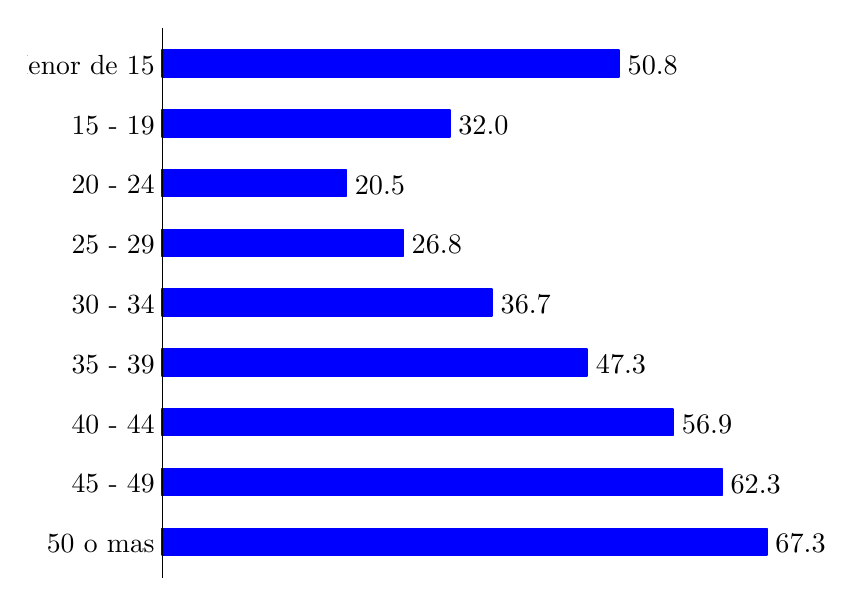
\begin{tikzpicture}[x=1pt,y=1pt]  % Created by tikzDevice version 0.10.1 on 2016-02-29 14:43:25
% !TEX encoding = UTF-8 Unicode
\definecolor{fillColor}{RGB}{255,255,255}
\path[use as bounding box,fill=fillColor,fill opacity=0.00] (0,0) rectangle (289.08,198.74);
\begin{scope}
\path[clip] (  0.00,  0.00) rectangle (289.08,198.74);

\path[] (  0.00,  0.00) rectangle (289.08,198.74);
\end{scope}
\begin{scope}
\path[clip] (  0.00,  0.00) rectangle (289.08,198.74);

\path[] ( 48.63,  0.00) rectangle (267.09,198.74);

\path[] ( 48.63, 12.96) --
	(267.09, 12.96);

\path[] ( 48.63, 34.56) --
	(267.09, 34.56);

\path[] ( 48.63, 56.17) --
	(267.09, 56.17);

\path[] ( 48.63, 77.77) --
	(267.09, 77.77);

\path[] ( 48.63, 99.37) --
	(267.09, 99.37);

\path[] ( 48.63,120.97) --
	(267.09,120.97);

\path[] ( 48.63,142.58) --
	(267.09,142.58);

\path[] ( 48.63,164.18) --
	(267.09,164.18);

\path[] ( 48.63,185.78) --
	(267.09,185.78);
\definecolor{drawColor}{RGB}{0,0,255}
\definecolor{fillColor}{RGB}{0,0,255}

\path[draw=drawColor,line width= 0.6pt,line join=round,fill=fillColor] ( 48.63,  8.10) rectangle (267.09, 17.82);

\path[draw=drawColor,line width= 0.6pt,line join=round,fill=fillColor] ( 48.63, 29.70) rectangle (250.88, 39.42);

\path[draw=drawColor,line width= 0.6pt,line join=round,fill=fillColor] ( 48.63, 51.31) rectangle (233.29, 61.03);

\path[draw=drawColor,line width= 0.6pt,line join=round,fill=fillColor] ( 48.63, 72.91) rectangle (202.21, 82.63);

\path[draw=drawColor,line width= 0.6pt,line join=round,fill=fillColor] ( 48.63, 94.51) rectangle (167.78,104.23);

\path[draw=drawColor,line width= 0.6pt,line join=round,fill=fillColor] ( 48.63,116.11) rectangle (135.64,125.83);

\path[draw=drawColor,line width= 0.6pt,line join=round,fill=fillColor] ( 48.63,137.72) rectangle (115.07,147.44);

\path[draw=drawColor,line width= 0.6pt,line join=round,fill=fillColor] ( 48.63,159.32) rectangle (152.49,169.04);

\path[draw=drawColor,line width= 0.6pt,line join=round,fill=fillColor] ( 48.63,180.92) rectangle (213.67,190.64);
\definecolor{drawColor}{RGB}{0,0,0}

\path[draw=drawColor,line width= 0.1pt,line join=round] ( 48.63,  0.00) -- ( 48.63,198.74);

\node[text=drawColor,anchor=base west,inner sep=0pt, outer sep=0pt, scale=  1.02] at (270.21,  8.99) {67.3};

\node[text=drawColor,anchor=base west,inner sep=0pt, outer sep=0pt, scale=  1.02] at (254.01, 30.59) {62.3};

\node[text=drawColor,anchor=base west,inner sep=0pt, outer sep=0pt, scale=  1.02] at (236.42, 52.20) {56.9};

\node[text=drawColor,anchor=base west,inner sep=0pt, outer sep=0pt, scale=  1.02] at (205.34, 73.80) {47.3};

\node[text=drawColor,anchor=base west,inner sep=0pt, outer sep=0pt, scale=  1.02] at (170.91, 95.40) {36.7};

\node[text=drawColor,anchor=base west,inner sep=0pt, outer sep=0pt, scale=  1.02] at (138.77,117.00) {26.8};

\node[text=drawColor,anchor=base west,inner sep=0pt, outer sep=0pt, scale=  1.02] at (118.20,138.61) {20.5};

\node[text=drawColor,anchor=base west,inner sep=0pt, outer sep=0pt, scale=  1.02] at (155.62,160.21) {32.0};

\node[text=drawColor,anchor=base west,inner sep=0pt, outer sep=0pt, scale=  1.02] at (216.80,181.81) {50.8};

\path[] ( 48.63,  0.00) rectangle (267.09,198.74);
\end{scope}
\begin{scope}
\path[clip] (  0.00,  0.00) rectangle (289.08,198.74);

\path[] ( 48.63,  0.00) --
	( 48.63,198.74);
\end{scope}
\begin{scope}
\path[clip] (  0.00,  0.00) rectangle (289.08,198.74);
\definecolor{drawColor}{RGB}{0,0,0}

\node[text=drawColor,anchor=base east,inner sep=0pt, outer sep=0pt, scale=  1.00] at ( 45.88,  9.05) {50 o mas};

\node[text=drawColor,anchor=base east,inner sep=0pt, outer sep=0pt, scale=  1.00] at ( 45.88, 30.66) {45 - 49};

\node[text=drawColor,anchor=base east,inner sep=0pt, outer sep=0pt, scale=  1.00] at ( 45.88, 52.26) {40 - 44};

\node[text=drawColor,anchor=base east,inner sep=0pt, outer sep=0pt, scale=  1.00] at ( 45.88, 73.86) {35 - 39};

\node[text=drawColor,anchor=base east,inner sep=0pt, outer sep=0pt, scale=  1.00] at ( 45.88, 95.46) {30 - 34};

\node[text=drawColor,anchor=base east,inner sep=0pt, outer sep=0pt, scale=  1.00] at ( 45.88,117.07) {25 - 29};

\node[text=drawColor,anchor=base east,inner sep=0pt, outer sep=0pt, scale=  1.00] at ( 45.88,138.67) {20 - 24};

\node[text=drawColor,anchor=base east,inner sep=0pt, outer sep=0pt, scale=  1.00] at ( 45.88,160.27) {15 - 19};

\node[text=drawColor,anchor=base east,inner sep=0pt, outer sep=0pt, scale=  1.00] at ( 45.88,181.87) {Menor de 15};
\end{scope}
\begin{scope}
\path[clip] (  0.00,  0.00) rectangle (289.08,198.74);

\path[] ( 45.88, 12.96) --
	( 48.63, 12.96);

\path[] ( 45.88, 34.56) --
	( 48.63, 34.56);

\path[] ( 45.88, 56.17) --
	( 48.63, 56.17);

\path[] ( 45.88, 77.77) --
	( 48.63, 77.77);

\path[] ( 45.88, 99.37) --
	( 48.63, 99.37);

\path[] ( 45.88,120.97) --
	( 48.63,120.97);

\path[] ( 45.88,142.58) --
	( 48.63,142.58);

\path[] ( 45.88,164.18) --
	( 48.63,164.18);

\path[] ( 45.88,185.78) --
	( 48.63,185.78);
\end{scope}
  \end{tikzpicture}}{Instituto Nacional de Estadística, de las Estadísticas Vitales 2014}




\cajita{Promedio de hijos}{Al realizar el análisis del número de hijos tenidos por las madres que tuvieron según el nivel de escolaridad de las madres, tuvieron un nacimiento en el 2014, aquellas sin ningún nivel de escolaridad tenían en promedio 3.6 hijos y las madres con nivel de posgrado, 1.6 hijos.}{Promedio de hijos tenidos por madre al momento del nuevo nacimiento, según su escolaridad}{República de Guatemala, 2014, en porcentaje}{\ \\[0mm]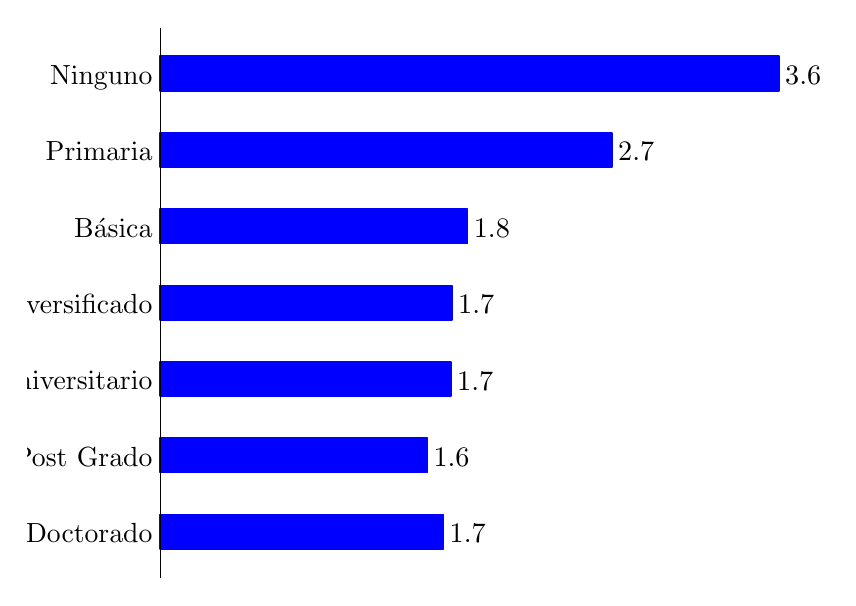
\begin{tikzpicture}[x=1pt,y=1pt]  % Created by tikzDevice version 0.10.1 on 2016-02-29 14:40:04
% !TEX encoding = UTF-8 Unicode
\definecolor{fillColor}{RGB}{255,255,255}
\path[use as bounding box,fill=fillColor,fill opacity=0.00] (0,0) rectangle (289.08,198.74);
\begin{scope}
\path[clip] (  0.00,  0.00) rectangle (289.08,198.74);

\path[] ( -0.00,  0.00) rectangle (289.08,198.74);
\end{scope}
\begin{scope}
\path[clip] (  0.00,  0.00) rectangle (289.08,198.74);

\path[] ( 47.80,  0.00) rectangle (271.48,198.74);

\path[] ( 47.80, 16.56) --
	(271.48, 16.56);

\path[] ( 47.80, 44.16) --
	(271.48, 44.16);

\path[] ( 47.80, 71.77) --
	(271.48, 71.77);

\path[] ( 47.80, 99.37) --
	(271.48, 99.37);

\path[] ( 47.80,126.97) --
	(271.48,126.97);

\path[] ( 47.80,154.58) --
	(271.48,154.58);

\path[] ( 47.80,182.18) --
	(271.48,182.18);
\definecolor{drawColor}{RGB}{0,0,255}
\definecolor{fillColor}{RGB}{0,0,255}

\path[draw=drawColor,line width= 0.6pt,line join=round,fill=fillColor] ( 47.80, 10.35) rectangle (150.28, 22.77);

\path[draw=drawColor,line width= 0.6pt,line join=round,fill=fillColor] ( 47.80, 37.95) rectangle (144.42, 50.38);

\path[draw=drawColor,line width= 0.6pt,line join=round,fill=fillColor] ( 47.80, 65.56) rectangle (152.95, 77.98);

\path[draw=drawColor,line width= 0.6pt,line join=round,fill=fillColor] ( 47.80, 93.16) rectangle (153.31,105.58);

\path[draw=drawColor,line width= 0.6pt,line join=round,fill=fillColor] ( 47.80,120.76) rectangle (158.98,133.19);

\path[draw=drawColor,line width= 0.6pt,line join=round,fill=fillColor] ( 47.80,148.37) rectangle (211.14,160.79);

\path[draw=drawColor,line width= 0.6pt,line join=round,fill=fillColor] ( 47.80,175.97) rectangle (271.48,188.39);
\definecolor{drawColor}{RGB}{0,0,0}

\path[draw=drawColor,line width= 0.1pt,line join=round] ( 47.80,  0.00) -- ( 47.80,198.74);

\node[text=drawColor,anchor=base west,inner sep=0pt, outer sep=0pt, scale=  1.02] at (152.51, 12.59) {1.7};

\node[text=drawColor,anchor=base west,inner sep=0pt, outer sep=0pt, scale=  1.02] at (146.66, 40.19) {1.6};

\node[text=drawColor,anchor=base west,inner sep=0pt, outer sep=0pt, scale=  1.02] at (155.19, 67.80) {1.7};

\node[text=drawColor,anchor=base west,inner sep=0pt, outer sep=0pt, scale=  1.02] at (155.55, 95.40) {1.7};

\node[text=drawColor,anchor=base west,inner sep=0pt, outer sep=0pt, scale=  1.02] at (161.22,123.00) {1.8};

\node[text=drawColor,anchor=base west,inner sep=0pt, outer sep=0pt, scale=  1.02] at (213.38,150.61) {2.7};

\node[text=drawColor,anchor=base west,inner sep=0pt, outer sep=0pt, scale=  1.02] at (273.72,178.21) {3.6};

\path[] ( 47.80,  0.00) rectangle (271.48,198.74);
\end{scope}
\begin{scope}
\path[clip] (  0.00,  0.00) rectangle (289.08,198.74);

\path[] ( 47.80,  0.00) --
	( 47.80,198.74);
\end{scope}
\begin{scope}
\path[clip] (  0.00,  0.00) rectangle (289.08,198.74);
\definecolor{drawColor}{RGB}{0,0,0}

\node[text=drawColor,anchor=base east,inner sep=0pt, outer sep=0pt, scale=  1.00] at ( 45.05, 12.65) {Doctorado};

\node[text=drawColor,anchor=base east,inner sep=0pt, outer sep=0pt, scale=  1.00] at ( 45.05, 40.26) {Post Grado};

\node[text=drawColor,anchor=base east,inner sep=0pt, outer sep=0pt, scale=  1.00] at ( 45.05, 67.86) {Universitario};

\node[text=drawColor,anchor=base east,inner sep=0pt, outer sep=0pt, scale=  1.00] at ( 45.05, 95.46) {Diversificado};

\node[text=drawColor,anchor=base east,inner sep=0pt, outer sep=0pt, scale=  1.00] at ( 45.05,123.07) {Básica};

\node[text=drawColor,anchor=base east,inner sep=0pt, outer sep=0pt, scale=  1.00] at ( 45.05,150.67) {Primaria};

\node[text=drawColor,anchor=base east,inner sep=0pt, outer sep=0pt, scale=  1.00] at ( 45.05,178.27) {Ninguno};
\end{scope}
\begin{scope}
\path[clip] (  0.00,  0.00) rectangle (289.08,198.74);

\path[] ( 45.05, 16.56) --
	( 47.80, 16.56);

\path[] ( 45.05, 44.16) --
	( 47.80, 44.16);

\path[] ( 45.05, 71.77) --
	( 47.80, 71.77);

\path[] ( 45.05, 99.37) --
	( 47.80, 99.37);

\path[] ( 45.05,126.97) --
	( 47.80,126.97);

\path[] ( 45.05,154.58) --
	( 47.80,154.58);

\path[] ( 45.05,182.18) --
	( 47.80,182.18);
\end{scope}
  \end{tikzpicture}}{Instituto Nacional de Estadística, de las Estadísticas Vitales 2014}

\cajita{Promedio de hijos de madres sin escolaridad}{Según los nacimientos reportados cada año, las madres sin ningún nivel de educación han tenido al momento del nuevo nacimiento, un promedio de 3.6 hijos, el cual no ha tenido mayor variación en los últimos 5 años.}{Promedio de hijos tenidos por madre sin educación,\\ al momento del nuevo nacimiento}{República de Guatemala, serie histórica, en porcentaje}{\ \\[0mm]\begin{tikzpicture}[x=1pt,y=1pt]  % Created by tikzDevice version 0.10.1 on 2016-02-29 14:40:32
% !TEX encoding = UTF-8 Unicode
\definecolor{fillColor}{RGB}{255,255,255}
\path[use as bounding box,fill=fillColor,fill opacity=0.00] (0,0) rectangle (289.08,198.74);
\begin{scope}
\path[clip] (  0.00,  0.00) rectangle (289.08,198.74);

\path[] (  0.00,  0.00) rectangle (289.08,198.74);
\end{scope}
\begin{scope}
\path[clip] (  0.00,  0.00) rectangle (289.08,198.74);

\path[] ( -4.90, 15.61) rectangle (280.54,191.48);

\path[] (  0.00, 52.34) --
	(280.54, 52.34);

\path[] (  0.00,109.79) --
	(280.54,109.79);

\path[] (  0.00,167.25) --
	(280.54,167.25);

\path[] (  0.00, 23.61) --
	(280.54, 23.61);

\path[] (  0.00, 81.06) --
	(280.54, 81.06);

\path[] (  0.00,138.52) --
	(280.54,138.52);

\path[] ( 28.04, 15.61) --
	( 28.04,191.48);

\path[] ( 82.93, 15.61) --
	( 82.93,191.48);

\path[] (137.82, 15.61) --
	(137.82,191.48);

\path[] (192.72, 15.61) --
	(192.72,191.48);

\path[] (247.61, 15.61) --
	(247.61,191.48);
\definecolor{drawColor}{RGB}{0,0,255}

\path[draw=drawColor,line width= 1.7pt,line join=round] ( 28.04,182.08) --
	( 82.93,179.87) --
	(137.82,183.49) --
	(192.72,178.74) --
	(247.61,175.17);
\definecolor{drawColor}{RGB}{0,0,0}

\node[text=drawColor,anchor=base,inner sep=0pt, outer sep=0pt, scale=  1.02] at ( 28.04,186.05) {3.8};

\node[text=drawColor,anchor=base,inner sep=0pt, outer sep=0pt, scale=  1.02] at ( 82.93,167.95) {3.7};

\node[text=drawColor,anchor=base,inner sep=0pt, outer sep=0pt, scale=  1.02] at (137.82,187.46) {3.8};

\node[text=drawColor,anchor=base west,inner sep=0pt, outer sep=0pt, scale=  1.02] at (192.72,182.71) {3.7};

\node[text=drawColor,anchor=base,inner sep=0pt, outer sep=0pt, scale=  1.02] at (247.61,163.26) {3.6};

\path[draw=drawColor,line width= 0.1pt,line join=round] (  0.00, 23.61) -- (280.54, 23.61);

\path[] ( -4.90, 15.61) rectangle (280.54,191.48);
\end{scope}
\begin{scope}
\path[clip] (  0.00,  0.00) rectangle (289.08,198.74);

\path[] (  0.00, 15.61) --
	(280.54, 15.61);
\end{scope}
\begin{scope}
\path[clip] (  0.00,  0.00) rectangle (289.08,198.74);

\path[] ( 28.04, 12.86) --
	( 28.04, 15.61);

\path[] ( 82.93, 12.86) --
	( 82.93, 15.61);

\path[] (137.82, 12.86) --
	(137.82, 15.61);

\path[] (192.72, 12.86) --
	(192.72, 15.61);

\path[] (247.61, 12.86) --
	(247.61, 15.61);
\end{scope}
\begin{scope}
\path[clip] (  0.00,  0.00) rectangle (289.08,198.74);
\definecolor{drawColor}{RGB}{0,0,0}

\node[text=drawColor,anchor=base,inner sep=0pt, outer sep=0pt, scale=  1.00] at ( 28.04,  2.85) {2010};

\node[text=drawColor,anchor=base,inner sep=0pt, outer sep=0pt, scale=  1.00] at ( 82.93,  2.85) {2011};

\node[text=drawColor,anchor=base,inner sep=0pt, outer sep=0pt, scale=  1.00] at (137.82,  2.85) {2012};

\node[text=drawColor,anchor=base,inner sep=0pt, outer sep=0pt, scale=  1.00] at (192.72,  2.85) {2013};

\node[text=drawColor,anchor=base,inner sep=0pt, outer sep=0pt, scale=  1.00] at (247.61,  2.85) {2014};
\end{scope}
  \end{tikzpicture}}{Instituto Nacional de Estadística, de las Estadísticas Vitales 2014}


\cajota{Promedio de hijos de madres sin escolaridad en los departamentos}{Según los nacimientos reportados en el 2014, las madres sin ningún nivel de escolaridad, tenían en promedio 3.6 hijos.
	
	 A nivel departamental, el mayor número de hijos en promedio en madres sin educación se dio en Quiché (4.1), Petén(4.0) y Sololá (4.0).}{Promedio de hijos tenidos por madre sin educación, al momento del nuevo nacimiento}{Por departamento, 2014, en porcentaje}{\includegraphics[width=52\cuadri]{graficas/vitales/Hoja8.pdf}}{Instituto Nacional de Estadística, de las Estadísticas Vitales 2014}



% % % % % Hoja 15

\cajita{Escolaridad de las madres y peso bajo en el recién nacido}{\textollamada{Se considera que el recién nacido tuvo peso bajo, cuando este es menor a 5.5 libras.} Al desagregar los nacimientos ocurridos en el 2014, de acuerdo a la escolaridad de la madre, se observa que en las madres sin escolaridad el 10.0\% tuvo peso bajo al nacer.
	
	En las  madres con post-grado, se observa el mayor porcentaje, aunque en términos absolutos estos fueron 9 de 56 nacimientos. }{Proporción de nacimientos con bajo peso, según la escolaridad de la madre}{República de Guatemala, año 2014, en porcentaje}{\ \\[0mm]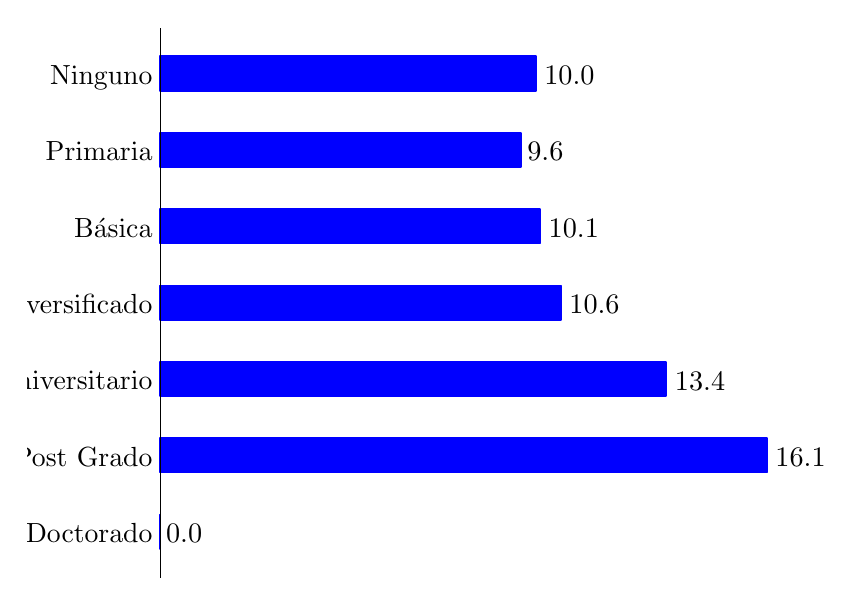
\begin{tikzpicture}[x=1pt,y=1pt]  % Created by tikzDevice version 0.10.1 on 2016-02-29 14:42:48
% !TEX encoding = UTF-8 Unicode
\definecolor{fillColor}{RGB}{255,255,255}
\path[use as bounding box,fill=fillColor,fill opacity=0.00] (0,0) rectangle (289.08,198.74);
\begin{scope}
\path[clip] (  0.00,  0.00) rectangle (289.08,198.74);

\path[] (  0.00,  0.00) rectangle (289.08,198.74);
\end{scope}
\begin{scope}
\path[clip] (  0.00,  0.00) rectangle (289.08,198.74);

\path[] ( 47.80,  0.00) rectangle (267.09,198.74);

\path[] ( 47.80, 16.56) --
	(267.09, 16.56);

\path[] ( 47.80, 44.16) --
	(267.09, 44.16);

\path[] ( 47.80, 71.77) --
	(267.09, 71.77);

\path[] ( 47.80, 99.37) --
	(267.09, 99.37);

\path[] ( 47.80,126.97) --
	(267.09,126.97);

\path[] ( 47.80,154.58) --
	(267.09,154.58);

\path[] ( 47.80,182.18) --
	(267.09,182.18);
\definecolor{drawColor}{RGB}{0,0,255}
\definecolor{fillColor}{RGB}{0,0,255}

\path[draw=drawColor,line width= 0.6pt,line join=round,fill=fillColor] ( 47.80, 10.35) rectangle ( 47.80, 22.77);

\path[draw=drawColor,line width= 0.6pt,line join=round,fill=fillColor] ( 47.80, 37.95) rectangle (267.09, 50.38);

\path[draw=drawColor,line width= 0.6pt,line join=round,fill=fillColor] ( 47.80, 65.56) rectangle (230.77, 77.98);

\path[draw=drawColor,line width= 0.6pt,line join=round,fill=fillColor] ( 47.80, 93.16) rectangle (192.63,105.58);

\path[draw=drawColor,line width= 0.6pt,line join=round,fill=fillColor] ( 47.80,120.76) rectangle (185.14,133.19);

\path[draw=drawColor,line width= 0.6pt,line join=round,fill=fillColor] ( 47.80,148.37) rectangle (178.32,160.79);

\path[draw=drawColor,line width= 0.6pt,line join=round,fill=fillColor] ( 47.80,175.97) rectangle (183.58,188.39);
\definecolor{drawColor}{RGB}{0,0,0}

\path[draw=drawColor,line width= 0.1pt,line join=round] ( 47.80,  0.00) -- ( 47.80,198.74);

\node[text=drawColor,anchor=base west,inner sep=0pt, outer sep=0pt, scale=  1.02] at ( 50.03, 12.59) {0.0};

\node[text=drawColor,anchor=base west,inner sep=0pt, outer sep=0pt, scale=  1.02] at (270.21, 40.19) {16.1};

\node[text=drawColor,anchor=base west,inner sep=0pt, outer sep=0pt, scale=  1.02] at (233.89, 67.80) {13.4};

\node[text=drawColor,anchor=base west,inner sep=0pt, outer sep=0pt, scale=  1.02] at (195.76, 95.40) {10.6};

\node[text=drawColor,anchor=base west,inner sep=0pt, outer sep=0pt, scale=  1.02] at (188.27,123.00) {10.1};

\node[text=drawColor,anchor=base west,inner sep=0pt, outer sep=0pt, scale=  1.02] at (180.56,150.61) {9.6};

\node[text=drawColor,anchor=base west,inner sep=0pt, outer sep=0pt, scale=  1.02] at (186.71,178.21) {10.0};

\path[] ( 47.80,  0.00) rectangle (267.09,198.74);
\end{scope}
\begin{scope}
\path[clip] (  0.00,  0.00) rectangle (289.08,198.74);

\path[] ( 47.80,  0.00) --
	( 47.80,198.74);
\end{scope}
\begin{scope}
\path[clip] (  0.00,  0.00) rectangle (289.08,198.74);
\definecolor{drawColor}{RGB}{0,0,0}

\node[text=drawColor,anchor=base east,inner sep=0pt, outer sep=0pt, scale=  1.00] at ( 45.05, 12.65) {Doctorado};

\node[text=drawColor,anchor=base east,inner sep=0pt, outer sep=0pt, scale=  1.00] at ( 45.05, 40.26) {Post Grado};

\node[text=drawColor,anchor=base east,inner sep=0pt, outer sep=0pt, scale=  1.00] at ( 45.05, 67.86) {Universitario};

\node[text=drawColor,anchor=base east,inner sep=0pt, outer sep=0pt, scale=  1.00] at ( 45.05, 95.46) {Diversificado};

\node[text=drawColor,anchor=base east,inner sep=0pt, outer sep=0pt, scale=  1.00] at ( 45.05,123.07) {Básica};

\node[text=drawColor,anchor=base east,inner sep=0pt, outer sep=0pt, scale=  1.00] at ( 45.05,150.67) {Primaria};

\node[text=drawColor,anchor=base east,inner sep=0pt, outer sep=0pt, scale=  1.00] at ( 45.05,178.27) {Ninguno};
\end{scope}
\begin{scope}
\path[clip] (  0.00,  0.00) rectangle (289.08,198.74);

\path[] ( 45.05, 16.56) --
	( 47.80, 16.56);

\path[] ( 45.05, 44.16) --
	( 47.80, 44.16);

\path[] ( 45.05, 71.77) --
	( 47.80, 71.77);

\path[] ( 45.05, 99.37) --
	( 47.80, 99.37);

\path[] ( 45.05,126.97) --
	( 47.80,126.97);

\path[] ( 45.05,154.58) --
	( 47.80,154.58);

\path[] ( 45.05,182.18) --
	( 47.80,182.18);
\end{scope}
  \end{tikzpicture}}{Instituto Nacional de Estadística, de las Estadísticas Vitales 2014}



% % % % Hoja17
\cajita{Madres sin escolaridad estado civil}{Al examinar los nacimientos de acuerdo al estado civil de las madres, se observa que el 31.5\% de las madres solteras no tenían ningún nivel de escolaridad. De las madres casadas, el 28.5\% y de las madres unidas el 60.2\%.}{Proporción de nacimientos en madres sin escolaridad según estado civil}{República de Guatemala, año 2014, en porcentaje}{\ \\[0mm]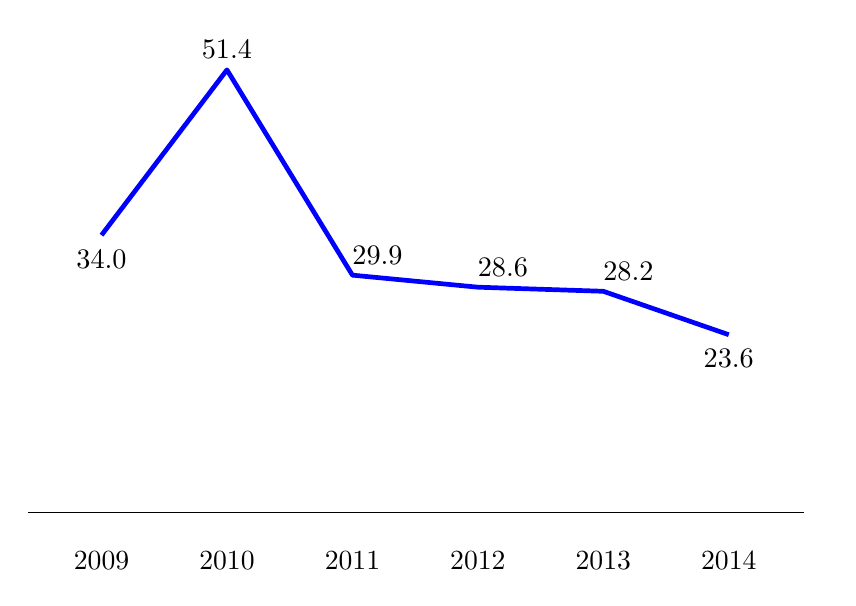
\begin{tikzpicture}[x=1pt,y=1pt]  % Created by tikzDevice version 0.10.1 on 2016-02-29 12:52:16
% !TEX encoding = UTF-8 Unicode
\definecolor{fillColor}{RGB}{255,255,255}
\path[use as bounding box,fill=fillColor,fill opacity=0.00] (0,0) rectangle (289.08,198.74);
\begin{scope}
\path[clip] (  0.00,  0.00) rectangle (289.08,198.74);

\path[] (  0.00,  0.00) rectangle (289.08,198.74);
\end{scope}
\begin{scope}
\path[clip] (  0.00,  0.00) rectangle (289.08,198.74);

\path[] ( -0.52, 15.61) rectangle (280.54,191.48);

\path[] (  0.00, 23.61) --
	(280.54, 23.61);

\path[] (  0.00, 58.09) --
	(280.54, 58.09);

\path[] (  0.00, 92.58) --
	(280.54, 92.58);

\path[] (  0.00,127.07) --
	(280.54,127.07);

\path[] (  0.00,161.56) --
	(280.54,161.56);

\path[] (  0.00, 40.85) --
	(280.54, 40.85);

\path[] (  0.00, 75.34) --
	(280.54, 75.34);

\path[] (  0.00,109.82) --
	(280.54,109.82);

\path[] (  0.00,144.31) --
	(280.54,144.31);

\path[] (  0.00,178.80) --
	(280.54,178.80);

\path[] ( 26.68, 15.61) --
	( 26.68,191.48);

\path[] ( 72.01, 15.61) --
	( 72.01,191.48);

\path[] (117.35, 15.61) --
	(117.35,191.48);

\path[] (162.68, 15.61) --
	(162.68,191.48);

\path[] (208.01, 15.61) --
	(208.01,191.48);

\path[] (253.34, 15.61) --
	(253.34,191.48);
\definecolor{drawColor}{RGB}{0,0,255}

\path[draw=drawColor,line width= 1.7pt,line join=round] ( 26.68,123.76) --
	( 72.01,183.49) --
	(117.35,109.31) --
	(162.68,104.96) --
	(208.01,103.48) --
	(253.34, 87.79);
\definecolor{drawColor}{RGB}{0,0,0}

\node[text=drawColor,anchor=base,inner sep=0pt, outer sep=0pt, scale=  1.02] at ( 26.68,111.84) {34.0};

\node[text=drawColor,anchor=base,inner sep=0pt, outer sep=0pt, scale=  1.02] at ( 72.01,187.46) {51.4};

\node[text=drawColor,anchor=base west,inner sep=0pt, outer sep=0pt, scale=  1.02] at (117.35,113.28) {29.9};

\node[text=drawColor,anchor=base west,inner sep=0pt, outer sep=0pt, scale=  1.02] at (162.68,108.93) {28.6};

\node[text=drawColor,anchor=base west,inner sep=0pt, outer sep=0pt, scale=  1.02] at (208.01,107.45) {28.2};

\node[text=drawColor,anchor=base,inner sep=0pt, outer sep=0pt, scale=  1.02] at (253.34, 75.87) {23.6};

\path[draw=drawColor,line width= 0.1pt,line join=round] (  0.00, 23.61) -- (280.54, 23.61);

\path[] ( -0.52, 15.61) rectangle (280.54,191.48);
\end{scope}
\begin{scope}
\path[clip] (  0.00,  0.00) rectangle (289.08,198.74);

\path[] (  0.00, 15.61) --
	(280.54, 15.61);
\end{scope}
\begin{scope}
\path[clip] (  0.00,  0.00) rectangle (289.08,198.74);

\path[] ( 26.68, 12.86) --
	( 26.68, 15.61);

\path[] ( 72.01, 12.86) --
	( 72.01, 15.61);

\path[] (117.35, 12.86) --
	(117.35, 15.61);

\path[] (162.68, 12.86) --
	(162.68, 15.61);

\path[] (208.01, 12.86) --
	(208.01, 15.61);

\path[] (253.34, 12.86) --
	(253.34, 15.61);
\end{scope}
\begin{scope}
\path[clip] (  0.00,  0.00) rectangle (289.08,198.74);
\definecolor{drawColor}{RGB}{0,0,0}

\node[text=drawColor,anchor=base,inner sep=0pt, outer sep=0pt, scale=  1.00] at ( 26.68,  2.85) {2009};

\node[text=drawColor,anchor=base,inner sep=0pt, outer sep=0pt, scale=  1.00] at ( 72.01,  2.85) {2010};

\node[text=drawColor,anchor=base,inner sep=0pt, outer sep=0pt, scale=  1.00] at (117.35,  2.85) {2011};

\node[text=drawColor,anchor=base,inner sep=0pt, outer sep=0pt, scale=  1.00] at (162.68,  2.85) {2012};

\node[text=drawColor,anchor=base,inner sep=0pt, outer sep=0pt, scale=  1.00] at (208.01,  2.85) {2013};

\node[text=drawColor,anchor=base,inner sep=0pt, outer sep=0pt, scale=  1.00] at (253.34,  2.85) {2014};
\end{scope}
  \end{tikzpicture}}{Instituto Nacional de Estadística, de las Estadísticas Vitales 2014}


\cajita{Madres que recibieron atención médica}{Al analizar el tipo de atención recibida al momento del parto, del total de nacimientos en madres con educación hasta nivel de grado, el 98.3\%  recibió asistencia médica
	
	Por otro lado, en el 2014, solo el 48.4\% de las madres sin educación tuvo este tipo de atención.}{Proporción de nacimientos que recibieron atención médica según nivel de escolaridad de la madre}{República de Guatemala, 2014, en porcentaje}{\ \\[0mm]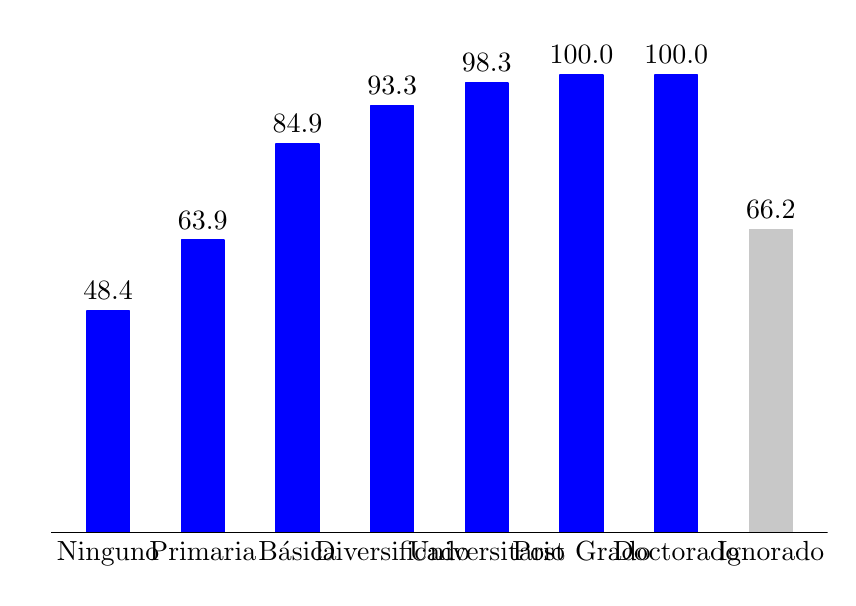
\begin{tikzpicture}[x=1pt,y=1pt]  % Created by tikzDevice version 0.8.1 on 2015-12-10 16:21:53
% !TEX encoding = UTF-8 Unicode
\definecolor{fillColor}{RGB}{255,255,255}
\path[use as bounding box,fill=fillColor,fill opacity=0.00] (0,0) rectangle (289.08,198.74);
\begin{scope}
\path[clip] (  0.00,  0.00) rectangle (289.08,198.74);

\path[] (  0.00,  0.00) rectangle (289.08,198.74);
\end{scope}
\begin{scope}
\path[clip] (  0.00,  0.00) rectangle (289.08,198.74);

\path[] (  8.54, 16.35) rectangle (289.08,181.67);

\path[] ( 29.06, 16.35) --
	( 29.06,181.67);

\path[] ( 63.28, 16.35) --
	( 63.28,181.67);

\path[] ( 97.49, 16.35) --
	( 97.49,181.67);

\path[] (131.70, 16.35) --
	(131.70,181.67);

\path[] (165.91, 16.35) --
	(165.91,181.67);

\path[] (200.13, 16.35) --
	(200.13,181.67);

\path[] (234.34, 16.35) --
	(234.34,181.67);

\path[] (268.55, 16.35) --
	(268.55,181.67);
\definecolor{drawColor}{RGB}{0,0,255}
\definecolor{fillColor}{RGB}{0,0,255}

\path[draw=drawColor,line width= 0.6pt,line join=round,fill=fillColor] ( 21.37, 16.35) rectangle ( 36.76, 96.39);

\path[draw=drawColor,line width= 0.6pt,line join=round,fill=fillColor] ( 55.58, 16.35) rectangle ( 70.97,121.92);

\path[draw=drawColor,line width= 0.6pt,line join=round,fill=fillColor] ( 89.79, 16.35) rectangle (105.19,156.76);

\path[draw=drawColor,line width= 0.6pt,line join=round,fill=fillColor] (124.00, 16.35) rectangle (139.40,170.65);

\path[draw=drawColor,line width= 0.6pt,line join=round,fill=fillColor] (158.22, 16.35) rectangle (173.61,178.78);

\path[draw=drawColor,line width= 0.6pt,line join=round,fill=fillColor] (192.43, 16.35) rectangle (207.82,181.67);

\path[draw=drawColor,line width= 0.6pt,line join=round,fill=fillColor] (226.64, 16.35) rectangle (242.04,181.67);
\definecolor{drawColor}{RGB}{200,200,200}
\definecolor{fillColor}{RGB}{200,200,200}

\path[draw=drawColor,line width= 0.6pt,line join=round,fill=fillColor] (260.85, 16.35) rectangle (276.25,125.80);
\definecolor{drawColor}{RGB}{0,0,0}

\path[draw=drawColor,line width= 0.1pt,line join=round] (  8.54, 16.35) -- (289.08, 16.35);

\node[text=drawColor,anchor=base,inner sep=0pt, outer sep=0pt, scale=  1.01] at ( 29.06,100.35) {48.4};

\node[text=drawColor,anchor=base,inner sep=0pt, outer sep=0pt, scale=  1.01] at ( 63.28,125.88) {63.9};

\node[text=drawColor,anchor=base,inner sep=0pt, outer sep=0pt, scale=  1.01] at ( 97.49,160.72) {84.9};

\node[text=drawColor,anchor=base,inner sep=0pt, outer sep=0pt, scale=  1.01] at (131.70,174.61) {93.3};

\node[text=drawColor,anchor=base,inner sep=0pt, outer sep=0pt, scale=  1.01] at (165.91,182.74) {98.3};

\node[text=drawColor,anchor=base,inner sep=0pt, outer sep=0pt, scale=  1.01] at (200.13,185.63) {100.0};

\node[text=drawColor,anchor=base,inner sep=0pt, outer sep=0pt, scale=  1.01] at (234.34,185.63) {100.0};

\node[text=drawColor,anchor=base,inner sep=0pt, outer sep=0pt, scale=  1.01] at (268.55,129.76) {66.2};

\path[] (  8.54, 16.35) rectangle (289.08,181.67);
\end{scope}
\begin{scope}
\path[clip] (  0.00,  0.00) rectangle (289.08,198.74);

\path[] (  8.54, 16.35) --
	(  8.54,181.67);
\end{scope}
\begin{scope}
\path[clip] (  0.00,  0.00) rectangle (289.08,198.74);

\path[] (  8.54, 16.35) --
	(289.08, 16.35);
\end{scope}
\begin{scope}
\path[clip] (  0.00,  0.00) rectangle (289.08,198.74);

\path[] ( 29.06, 12.08) --
	( 29.06, 16.35);

\path[] ( 63.28, 12.08) --
	( 63.28, 16.35);

\path[] ( 97.49, 12.08) --
	( 97.49, 16.35);

\path[] (131.70, 12.08) --
	(131.70, 16.35);

\path[] (165.91, 12.08) --
	(165.91, 16.35);

\path[] (200.13, 12.08) --
	(200.13, 16.35);

\path[] (234.34, 12.08) --
	(234.34, 16.35);

\path[] (268.55, 12.08) --
	(268.55, 16.35);
\end{scope}
\begin{scope}
\path[clip] (  0.00,  0.00) rectangle (289.08,198.74);
\definecolor{drawColor}{RGB}{0,0,0}

\node[text=drawColor,anchor=base,inner sep=0pt, outer sep=0pt, scale=  1.00] at ( 29.06,  6.04) {Ninguno};

\node[text=drawColor,anchor=base,inner sep=0pt, outer sep=0pt, scale=  1.00] at ( 63.28,  6.04) {Primaria};

\node[text=drawColor,anchor=base,inner sep=0pt, outer sep=0pt, scale=  1.00] at ( 97.49,  6.04) {Básica};

\node[text=drawColor,anchor=base,inner sep=0pt, outer sep=0pt, scale=  1.00] at (131.70,  6.04) {Diversificado};

\node[text=drawColor,anchor=base,inner sep=0pt, outer sep=0pt, scale=  1.00] at (165.91,  6.04) {Universitario};

\node[text=drawColor,anchor=base,inner sep=0pt, outer sep=0pt, scale=  1.00] at (200.13,  6.04) {Post Grado};

\node[text=drawColor,anchor=base,inner sep=0pt, outer sep=0pt, scale=  1.00] at (234.34,  6.04) {Doctorado};

\node[text=drawColor,anchor=base,inner sep=0pt, outer sep=0pt, scale=  1.00] at (268.55,  6.04) {Ignorado};
\end{scope}
  \end{tikzpicture}}{Instituto Nacional de Estadística, de las Estadísticas Vitales 2014}

\cajita{Madres sin escolaridad que recibieron atención médica}{La tendencia de los nacimientos en madres sin educación que reciben atención médica ha sido ascendente, sin embargo el mayor crecimiento se observa entre el 2013 y 2014.
	
	 En referencia al 2010, hubo un aumento en 14.3 puntos porcentuales.}{Proporción de nacimientos en madres sin educación, que recibieron atención médica}{República de Guatemala, serie histórica, en porcentaje}{\ \\[0mm]\begin{tikzpicture}[x=1pt,y=1pt]  % Created by tikzDevice version 0.10.1 on 2016-02-29 14:41:35
% !TEX encoding = UTF-8 Unicode
\definecolor{fillColor}{RGB}{255,255,255}
\path[use as bounding box,fill=fillColor,fill opacity=0.00] (0,0) rectangle (289.08,198.74);
\begin{scope}
\path[clip] (  0.00,  0.00) rectangle (289.08,198.74);

\path[] (  0.00,  0.00) rectangle (289.08,198.74);
\end{scope}
\begin{scope}
\path[clip] (  0.00,  0.00) rectangle (289.08,198.74);

\path[] ( -0.52, 15.61) rectangle (280.54,191.48);

\path[] (  0.00, 37.46) --
	(280.54, 37.46);

\path[] (  0.00, 72.10) --
	(280.54, 72.10);

\path[] (  0.00,106.74) --
	(280.54,106.74);

\path[] (  0.00,141.37) --
	(280.54,141.37);

\path[] (  0.00,176.01) --
	(280.54,176.01);

\path[] (  0.00, 20.14) --
	(280.54, 20.14);

\path[] (  0.00, 54.78) --
	(280.54, 54.78);

\path[] (  0.00, 89.42) --
	(280.54, 89.42);

\path[] (  0.00,124.05) --
	(280.54,124.05);

\path[] (  0.00,158.69) --
	(280.54,158.69);

\path[] ( 31.91, 15.61) --
	( 31.91,191.48);

\path[] ( 85.96, 15.61) --
	( 85.96,191.48);

\path[] (140.01, 15.61) --
	(140.01,191.48);

\path[] (194.06, 15.61) --
	(194.06,191.48);

\path[] (248.11, 15.61) --
	(248.11,191.48);
\definecolor{drawColor}{RGB}{0,0,255}

\path[draw=drawColor,line width= 1.7pt,line join=round] ( 31.91,138.26) --
	( 85.96,151.77) --
	(140.01,154.19) --
	(194.06,167.70) --
	(248.11,183.49);
\definecolor{drawColor}{RGB}{0,0,0}

\node[text=drawColor,anchor=base,inner sep=0pt, outer sep=0pt, scale=  1.02] at ( 31.91,126.34) {34.1};

\node[text=drawColor,anchor=base east,inner sep=0pt, outer sep=0pt, scale=  1.02] at ( 82.83,151.77) {38.0};

\node[text=drawColor,anchor=base east,inner sep=0pt, outer sep=0pt, scale=  1.02] at (136.88,154.19) {38.7};

\node[text=drawColor,anchor=base east,inner sep=0pt, outer sep=0pt, scale=  1.02] at (190.94,167.70) {42.6};

\node[text=drawColor,anchor=base,inner sep=0pt, outer sep=0pt, scale=  1.02] at (248.11,187.46) {47.2};

\path[draw=drawColor,line width= 0.1pt,line join=round] (  0.00, 23.61) -- (280.54, 23.61);

\path[] ( -0.52, 15.61) rectangle (280.54,191.48);
\end{scope}
\begin{scope}
\path[clip] (  0.00,  0.00) rectangle (289.08,198.74);

\path[] (  0.00, 15.61) --
	(280.54, 15.61);
\end{scope}
\begin{scope}
\path[clip] (  0.00,  0.00) rectangle (289.08,198.74);

\path[] ( 31.91, 12.86) --
	( 31.91, 15.61);

\path[] ( 85.96, 12.86) --
	( 85.96, 15.61);

\path[] (140.01, 12.86) --
	(140.01, 15.61);

\path[] (194.06, 12.86) --
	(194.06, 15.61);

\path[] (248.11, 12.86) --
	(248.11, 15.61);
\end{scope}
\begin{scope}
\path[clip] (  0.00,  0.00) rectangle (289.08,198.74);
\definecolor{drawColor}{RGB}{0,0,0}

\node[text=drawColor,anchor=base,inner sep=0pt, outer sep=0pt, scale=  1.00] at ( 31.91,  2.85) {2010};

\node[text=drawColor,anchor=base,inner sep=0pt, outer sep=0pt, scale=  1.00] at ( 85.96,  2.85) {2011};

\node[text=drawColor,anchor=base,inner sep=0pt, outer sep=0pt, scale=  1.00] at (140.01,  2.85) {2012};

\node[text=drawColor,anchor=base,inner sep=0pt, outer sep=0pt, scale=  1.00] at (194.06,  2.85) {2013};

\node[text=drawColor,anchor=base,inner sep=0pt, outer sep=0pt, scale=  1.00] at (248.11,  2.85) {2014};
\end{scope}
  \end{tikzpicture}}{Instituto Nacional de Estadística, de las Estadísticas Vitales 2014}


\cajota{Madres sin escolaridad que recibieron atención médica\newline en los departamentos}{Al analizar los nacimientos según el departamento de ocurrencia, de las madres sin ningún nivel de educación, se observa que los mayores porcentajes se dieron en Escuintla (87.3\%), Sacatepéquez (85.0\%) y Guatemala (80.9\%).
	
	En los departamentos de Huehuetenango, Totonicapán y Quiché se observaron los menores porcentajes de madres sin escolaridad que recibieron asistencia médica, siendo de 22.2\%, 28.1\% y 28.9\% respectivamente.}{Proporción de nacimientos de madres sin escolaridad que recibieron atención médica}{Por departamento de ocurrencia, 2014, en porcentaje}{\includegraphics[width=52\cuadri]{graficas/vitales/Hoja11.pdf}}{Instituto Nacional de Estadística, de las Estadísticas Vitales 2014}


\cajita{Nacimientos ocurridos en centro médico, según escolaridad la madre}{\textollamada{Incluye los nacimientos ocurridos en: hospital privado, hospital público, centro de salud e IGSS} Los nacimientos ocurridos en el 2014, más del 95\% de las madres con educación superior recibió atención en un centro médico.
	
	Por otro lado, solo el 47.6\% de las madres sin educación tuvo atención médica en este tipo de centro.}{Proporción de nacimientos que ocurrieron en centro médico, según el nivel de escolaridad de la madre}{República de Guatemala, 2014, en porcentaje}{\ \\[0mm]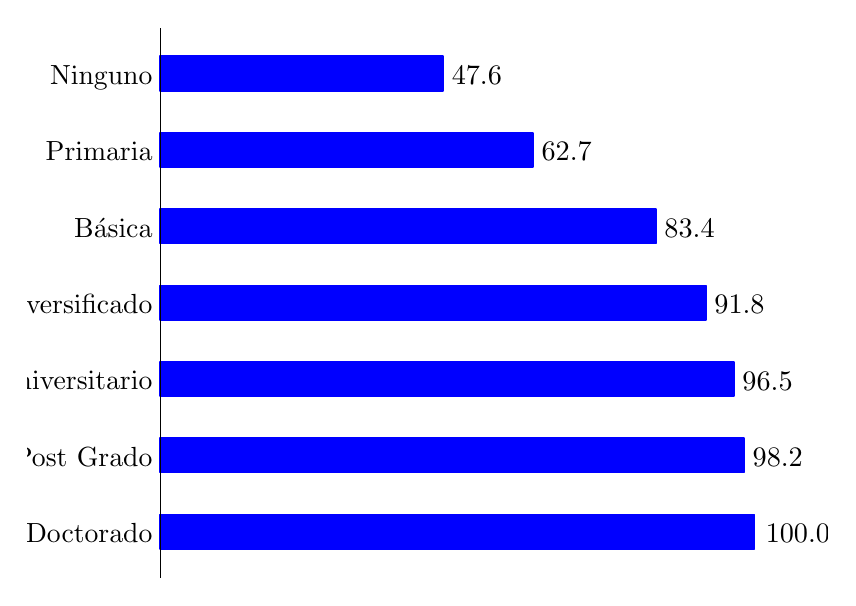
\begin{tikzpicture}[x=1pt,y=1pt]  % Created by tikzDevice version 0.10.1 on 2016-02-29 14:41:49
% !TEX encoding = UTF-8 Unicode
\definecolor{fillColor}{RGB}{255,255,255}
\path[use as bounding box,fill=fillColor,fill opacity=0.00] (0,0) rectangle (289.08,198.74);
\begin{scope}
\path[clip] (  0.00,  0.00) rectangle (289.08,198.74);

\path[] (  0.00,  0.00) rectangle (289.08,198.74);
\end{scope}
\begin{scope}
\path[clip] (  0.00,  0.00) rectangle (289.08,198.74);

\path[] ( 47.80,  0.00) rectangle (262.69,198.74);

\path[] ( 47.80, 16.56) --
	(262.69, 16.56);

\path[] ( 47.80, 44.16) --
	(262.69, 44.16);

\path[] ( 47.80, 71.77) --
	(262.69, 71.77);

\path[] ( 47.80, 99.37) --
	(262.69, 99.37);

\path[] ( 47.80,126.97) --
	(262.69,126.97);

\path[] ( 47.80,154.58) --
	(262.69,154.58);

\path[] ( 47.80,182.18) --
	(262.69,182.18);
\definecolor{drawColor}{RGB}{0,0,255}
\definecolor{fillColor}{RGB}{0,0,255}

\path[draw=drawColor,line width= 0.6pt,line join=round,fill=fillColor] ( 47.80, 10.35) rectangle (262.69, 22.77);

\path[draw=drawColor,line width= 0.6pt,line join=round,fill=fillColor] ( 47.80, 37.95) rectangle (258.85, 50.38);

\path[draw=drawColor,line width= 0.6pt,line join=round,fill=fillColor] ( 47.80, 65.56) rectangle (255.18, 77.98);

\path[draw=drawColor,line width= 0.6pt,line join=round,fill=fillColor] ( 47.80, 93.16) rectangle (245.02,105.58);

\path[draw=drawColor,line width= 0.6pt,line join=round,fill=fillColor] ( 47.80,120.76) rectangle (226.97,133.19);

\path[draw=drawColor,line width= 0.6pt,line join=round,fill=fillColor] ( 47.80,148.37) rectangle (182.58,160.79);

\path[draw=drawColor,line width= 0.6pt,line join=round,fill=fillColor] ( 47.80,175.97) rectangle (150.11,188.39);
\definecolor{drawColor}{RGB}{0,0,0}

\path[draw=drawColor,line width= 0.1pt,line join=round] ( 47.80,  0.00) -- ( 47.80,198.74);

\node[text=drawColor,anchor=base west,inner sep=0pt, outer sep=0pt, scale=  1.02] at (266.71, 12.59) {100.0};

\node[text=drawColor,anchor=base west,inner sep=0pt, outer sep=0pt, scale=  1.02] at (261.98, 40.19) {98.2};

\node[text=drawColor,anchor=base west,inner sep=0pt, outer sep=0pt, scale=  1.02] at (258.30, 67.80) {96.5};

\node[text=drawColor,anchor=base west,inner sep=0pt, outer sep=0pt, scale=  1.02] at (248.15, 95.40) {91.8};

\node[text=drawColor,anchor=base west,inner sep=0pt, outer sep=0pt, scale=  1.02] at (230.10,123.00) {83.4};

\node[text=drawColor,anchor=base west,inner sep=0pt, outer sep=0pt, scale=  1.02] at (185.71,150.61) {62.7};

\node[text=drawColor,anchor=base west,inner sep=0pt, outer sep=0pt, scale=  1.02] at (153.24,178.21) {47.6};

\path[] ( 47.80,  0.00) rectangle (262.69,198.74);
\end{scope}
\begin{scope}
\path[clip] (  0.00,  0.00) rectangle (289.08,198.74);

\path[] ( 47.80,  0.00) --
	( 47.80,198.74);
\end{scope}
\begin{scope}
\path[clip] (  0.00,  0.00) rectangle (289.08,198.74);
\definecolor{drawColor}{RGB}{0,0,0}

\node[text=drawColor,anchor=base east,inner sep=0pt, outer sep=0pt, scale=  1.00] at ( 45.05, 12.65) {Doctorado};

\node[text=drawColor,anchor=base east,inner sep=0pt, outer sep=0pt, scale=  1.00] at ( 45.05, 40.26) {Post Grado};

\node[text=drawColor,anchor=base east,inner sep=0pt, outer sep=0pt, scale=  1.00] at ( 45.05, 67.86) {Universitario};

\node[text=drawColor,anchor=base east,inner sep=0pt, outer sep=0pt, scale=  1.00] at ( 45.05, 95.46) {Diversificado};

\node[text=drawColor,anchor=base east,inner sep=0pt, outer sep=0pt, scale=  1.00] at ( 45.05,123.07) {Básica};

\node[text=drawColor,anchor=base east,inner sep=0pt, outer sep=0pt, scale=  1.00] at ( 45.05,150.67) {Primaria};

\node[text=drawColor,anchor=base east,inner sep=0pt, outer sep=0pt, scale=  1.00] at ( 45.05,178.27) {Ninguno};
\end{scope}
\begin{scope}
\path[clip] (  0.00,  0.00) rectangle (289.08,198.74);

\path[] ( 45.05, 16.56) --
	( 47.80, 16.56);

\path[] ( 45.05, 44.16) --
	( 47.80, 44.16);

\path[] ( 45.05, 71.77) --
	( 47.80, 71.77);

\path[] ( 45.05, 99.37) --
	( 47.80, 99.37);

\path[] ( 45.05,126.97) --
	( 47.80,126.97);

\path[] ( 45.05,154.58) --
	( 47.80,154.58);

\path[] ( 45.05,182.18) --
	( 47.80,182.18);
\end{scope}
  \end{tikzpicture}}{Instituto Nacional de Estadística, de las Estadísticas Vitales 2014}

\cajita{Nacimientos ocurridos en centro médico, madres sin escolaridad}{La tendencia de los nacimientos en madres sin educación que recibieron atención en un centro médico ha sido ascendente, sin embargo el mayor crecimiento se observó entre el 2012 y 2013.
	
	En referencia al 2010, hubo un aumento en 13.4 puntos porcentuales.}{Proporción de nacimientos en madres sin escolaridad, que ocurrieron en centros de atención médica}{República de Guatemala, serie histórica, en porcentaje}{\ \\[0mm]\begin{tikzpicture}[x=1pt,y=1pt]  % Created by tikzDevice version 0.8.1 on 2015-12-10 16:21:53
% !TEX encoding = UTF-8 Unicode
\definecolor{fillColor}{RGB}{255,255,255}
\path[use as bounding box,fill=fillColor,fill opacity=0.00] (0,0) rectangle (289.08,198.74);
\begin{scope}
\path[clip] (  0.00,  0.00) rectangle (289.08,198.74);

\path[] (  0.00,  0.00) rectangle (289.08,198.74);
\end{scope}
\begin{scope}
\path[clip] (  0.00,  0.00) rectangle (289.08,198.74);

\path[] (  1.64, 17.78) rectangle (280.54,191.48);

\path[] (  1.64, 42.25) --
	(280.54, 42.25);

\path[] (  1.64, 75.42) --
	(280.54, 75.42);

\path[] (  1.64,108.59) --
	(280.54,108.59);

\path[] (  1.64,141.76) --
	(280.54,141.76);

\path[] (  1.64,174.92) --
	(280.54,174.92);

\path[] (  1.64, 25.67) --
	(280.54, 25.67);

\path[] (  1.64, 58.84) --
	(280.54, 58.84);

\path[] (  1.64, 92.01) --
	(280.54, 92.01);

\path[] (  1.64,125.17) --
	(280.54,125.17);

\path[] (  1.64,158.34) --
	(280.54,158.34);

\path[] ( 33.83, 17.78) --
	( 33.83,191.48);

\path[] ( 87.46, 17.78) --
	( 87.46,191.48);

\path[] (141.09, 17.78) --
	(141.09,191.48);

\path[] (194.73, 17.78) --
	(194.73,191.48);

\path[] (248.36, 17.78) --
	(248.36,191.48);
\definecolor{drawColor}{RGB}{0,0,255}

\path[draw=drawColor,line width= 1.7pt,line join=round] ( 33.83,139.10) --
	( 87.46,152.37) --
	(141.09,154.36) --
	(194.73,169.62) --
	(248.36,183.59);
\definecolor{drawColor}{RGB}{0,0,0}

\node[text=drawColor,anchor=base,inner sep=0pt, outer sep=0pt, scale=  1.01] at ( 33.83,127.23) {34.2};

\node[text=drawColor,anchor=base east,inner sep=0pt, outer sep=0pt, scale=  1.01] at ( 84.34,152.37) {38.2};

\node[text=drawColor,anchor=base east,inner sep=0pt, outer sep=0pt, scale=  1.01] at (137.98,154.36) {38.8};

\node[text=drawColor,anchor=base east,inner sep=0pt, outer sep=0pt, scale=  1.01] at (191.61,169.62) {43.4};

\node[text=drawColor,anchor=base,inner sep=0pt, outer sep=0pt, scale=  1.01] at (248.36,187.54) {47.6};

\path[draw=drawColor,line width= 0.1pt,line join=round] (  1.64, 25.67) -- (280.54, 25.67);

\path[] (  1.64, 17.78) rectangle (280.54,191.48);
\end{scope}
\begin{scope}
\path[clip] (  0.00,  0.00) rectangle (289.08,198.74);

\path[] (  1.64, 17.78) --
	(  1.64,191.48);
\end{scope}
\begin{scope}
\path[clip] (  0.00,  0.00) rectangle (289.08,198.74);

\path[] (  0.00, 25.67) --
	(  1.64, 25.67);

\path[] (  0.00, 58.84) --
	(  1.64, 58.84);

\path[] (  0.00, 92.01) --
	(  1.64, 92.01);

\path[] (  0.00,125.17) --
	(  1.64,125.17);

\path[] (  0.00,158.34) --
	(  1.64,158.34);
\end{scope}
\begin{scope}
\path[clip] (  0.00,  0.00) rectangle (289.08,198.74);

\path[] (  1.64, 17.78) --
	(280.54, 17.78);
\end{scope}
\begin{scope}
\path[clip] (  0.00,  0.00) rectangle (289.08,198.74);

\path[] ( 33.83, 13.51) --
	( 33.83, 17.78);

\path[] ( 87.46, 13.51) --
	( 87.46, 17.78);

\path[] (141.09, 13.51) --
	(141.09, 17.78);

\path[] (194.73, 13.51) --
	(194.73, 17.78);

\path[] (248.36, 13.51) --
	(248.36, 17.78);
\end{scope}
\begin{scope}
\path[clip] (  0.00,  0.00) rectangle (289.08,198.74);
\definecolor{drawColor}{RGB}{0,0,0}

\node[text=drawColor,anchor=base,inner sep=0pt, outer sep=0pt, scale=  1.00] at ( 33.83,  2.85) {2010};

\node[text=drawColor,anchor=base,inner sep=0pt, outer sep=0pt, scale=  1.00] at ( 87.46,  2.85) {2011};

\node[text=drawColor,anchor=base,inner sep=0pt, outer sep=0pt, scale=  1.00] at (141.09,  2.85) {2012};

\node[text=drawColor,anchor=base,inner sep=0pt, outer sep=0pt, scale=  1.00] at (194.73,  2.85) {2013};

\node[text=drawColor,anchor=base,inner sep=0pt, outer sep=0pt, scale=  1.00] at (248.36,  2.85) {2014};
\end{scope}
  \end{tikzpicture}}{Instituto Nacional de Estadística, de las Estadísticas Vitales 2014}

\cajota{Madres sin escolaridad que recibieron atención médica\newline en los departamentos}{Al realizar el análisis en los departamentos de ocurrencia de los nacimientos, en madres sin ningún nivel de escolaridad, se observó que en Escuintla, Sacatepéquez y Guatemala se dio el mayor porcentaje de partos que se realizaron en un centro médico, siendo del 86.4\%, 84.7\% y 79.5\%, respectivamente.
	
	Los departamentos con las  menores proporciones fueron Quiché, Totonicapán y Huehuetenango.}{Nacimientos en madres sin educación que recibieron atención médica}{Por departamento de ocurrencia,2014, en porcentaje}{\includegraphics[width=52\cuadri]{graficas/vitales/Hoja14.pdf}}{Instituto Nacional de Estadística, de las Estadísticas Vitales 2014}




% % % % Hoja18
\cajita{Escolaridad del padre}{En relación a la escolaridad de los padres, de los nacimientos ocurridos en el 2014, el 39.0\% tenía algún grado de primaria y el 15.1\% no tenía ningún nivel de escolaridad.
	
	Se observaron 105 padres con nivel de posgrado y 8 con nivel de doctorado, los cuales representan menos del 1\%.}{Distribución porcentual de nacimientos según escolaridad del padre}{República de Guatemala, año 2014, en porcentaje}{\ \\[0mm]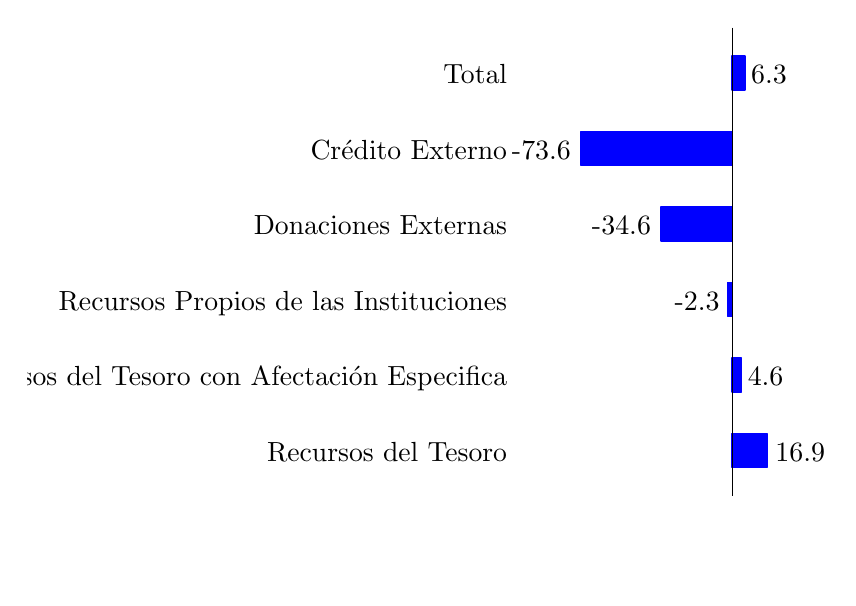
\begin{tikzpicture}[x=1pt,y=1pt]  % Created by tikzDevice version 0.7.0 on 2015-08-28 16:35:09
% !TEX encoding = UTF-8 Unicode
\definecolor[named]{fillColor}{rgb}{1.00,1.00,1.00}
\path[use as bounding box,fill=fillColor,fill opacity=0.00] (0,0) rectangle (289.08,198.74);
\begin{scope}
\path[clip] (  0.00,  0.00) rectangle (289.08,198.74);
\definecolor[named]{drawColor}{rgb}{1.00,1.00,1.00}

\path[draw=drawColor,line width= 0.6pt,line join=round,line cap=round] (  0.00,  0.00) rectangle (289.08,198.74);
\end{scope}
\begin{scope}
\path[clip] (  0.00,  0.00) rectangle (289.08,198.74);

\path[] (199.99, 29.60) rectangle (267.09,198.74);

\path[] (199.99, 45.97) --
	(267.09, 45.97);

\path[] (199.99, 73.25) --
	(267.09, 73.25);

\path[] (199.99,100.53) --
	(267.09,100.53);

\path[] (199.99,127.81) --
	(267.09,127.81);

\path[] (199.99,155.09) --
	(267.09,155.09);

\path[] (199.99,182.37) --
	(267.09,182.37);
\definecolor[named]{drawColor}{rgb}{0.00,0.00,1.00}
\definecolor[named]{fillColor}{rgb}{0.00,0.00,1.00}

\path[draw=drawColor,line width= 0.6pt,line join=round,fill=fillColor] (254.56, 39.83) rectangle (267.09, 52.11);

\path[draw=drawColor,line width= 0.6pt,line join=round,fill=fillColor] (254.56, 67.11) rectangle (257.97, 79.39);

\path[draw=drawColor,line width= 0.6pt,line join=round,fill=fillColor] (252.85, 94.39) rectangle (254.56,106.67);

\path[draw=drawColor,line width= 0.6pt,line join=round,fill=fillColor] (228.90,121.67) rectangle (254.56,133.95);

\path[draw=drawColor,line width= 0.6pt,line join=round,fill=fillColor] (199.99,148.95) rectangle (254.56,161.23);

\path[draw=drawColor,line width= 0.6pt,line join=round,fill=fillColor] (254.56,176.24) rectangle (259.23,188.51);
\definecolor[named]{drawColor}{rgb}{0.00,0.00,0.00}
\definecolor[named]{fillColor}{rgb}{0.00,0.00,0.00}

\path[draw=drawColor,line width= 0.1pt,line join=round,fill=fillColor] (254.56, 29.60) -- (254.56,198.74);

\node[text=drawColor,anchor=base west,inner sep=0pt, outer sep=0pt, scale=  1.01] at (270.20, 42.01) {16.9};

\node[text=drawColor,anchor=base west,inner sep=0pt, outer sep=0pt, scale=  1.01] at (260.20, 69.29) {4.6};

\node[text=drawColor,anchor=base east,inner sep=0pt, outer sep=0pt, scale=  1.01] at (250.06, 96.57) {-2.3};

\node[text=drawColor,anchor=base east,inner sep=0pt, outer sep=0pt, scale=  1.01] at (225.23,123.86) {-34.6};

\node[text=drawColor,anchor=base east,inner sep=0pt, outer sep=0pt, scale=  1.01] at (196.31,151.14) {-73.6};

\node[text=drawColor,anchor=base west,inner sep=0pt, outer sep=0pt, scale=  1.01] at (261.46,178.42) {6.3};
\end{scope}
\begin{scope}
\path[clip] (  0.00,  0.00) rectangle (289.08,198.74);

\path[] (199.99, 29.60) --
	(199.99,198.74);
\end{scope}
\begin{scope}
\path[clip] (  0.00,  0.00) rectangle (289.08,198.74);
\definecolor[named]{drawColor}{rgb}{0.00,0.00,0.00}

\node[text=drawColor,anchor=base east,inner sep=0pt, outer sep=0pt, scale=  1.00] at (173.23, 42.06) {Recursos del Tesoro};

\node[text=drawColor,anchor=base east,inner sep=0pt, outer sep=0pt, scale=  1.00] at (173.23, 69.34) {Recursos del Tesoro con Afectaci\'on Especifica};

\node[text=drawColor,anchor=base east,inner sep=0pt, outer sep=0pt, scale=  1.00] at (173.23, 96.62) {Recursos Propios de las Instituciones};

\node[text=drawColor,anchor=base east,inner sep=0pt, outer sep=0pt, scale=  1.00] at (173.23,123.90) {Donaciones Externas};

\node[text=drawColor,anchor=base east,inner sep=0pt, outer sep=0pt, scale=  1.00] at (173.23,151.18) {Cr\'edito Externo};

\node[text=drawColor,anchor=base east,inner sep=0pt, outer sep=0pt, scale=  1.00] at (173.23,178.47) {Total};
\end{scope}
\begin{scope}
\path[clip] (  0.00,  0.00) rectangle (289.08,198.74);

\path[] (173.23, 45.97) --
	(177.50, 45.97);

\path[] (173.23, 73.25) --
	(177.50, 73.25);

\path[] (173.23,100.53) --
	(177.50,100.53);

\path[] (173.23,127.81) --
	(177.50,127.81);

\path[] (173.23,155.09) --
	(177.50,155.09);

\path[] (173.23,182.37) --
	(177.50,182.37);
\end{scope}
\begin{scope}
\path[clip] (  0.00,  0.00) rectangle (289.08,198.74);

\path[] (199.99, 29.60) --
	(267.09, 29.60);
\end{scope}
  \end{tikzpicture}}{Instituto Nacional de Estadística, de las Estadísticas Vitales 2014}




% % % % Hoja19
\cajita{Padres sin escolaridad según estado civil}{De acuerdo a la escolaridad de los padres de los nacimientos ocurridos en el 2014, el 19.6\% de los padres solteros no tenían  ningún nivel de educación, el 15.1\% de los casados estaban con la misa situación escolar y por el lado de los unidos el 34.0\%.}{Proporción de nacimientos con padre sin escolaridad, según estado civil}{República de Guatemala, año 2014, en porcentaje}{\ \\[0mm]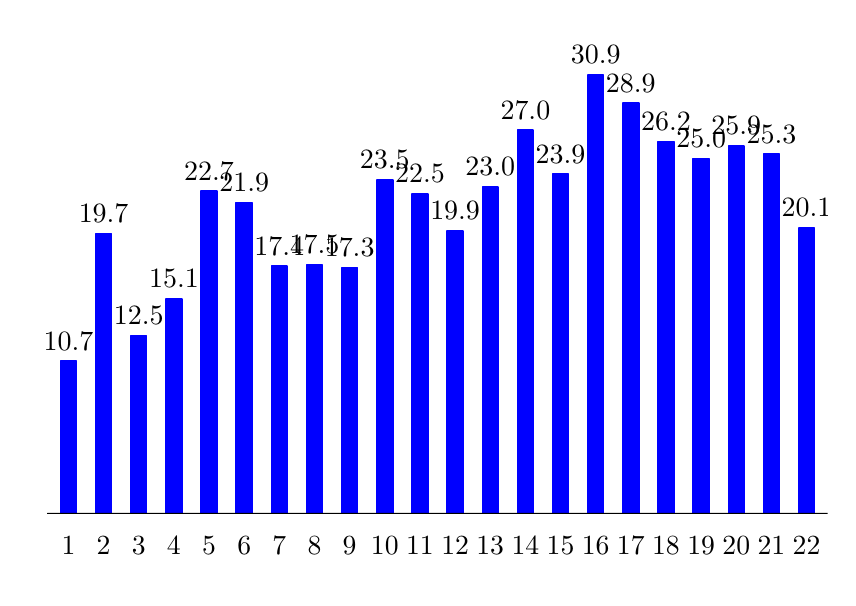
\begin{tikzpicture}[x=1pt,y=1pt]  % Created by tikzDevice version 0.7.0 on 2015-08-28 13:07:43
% !TEX encoding = UTF-8 Unicode
\definecolor[named]{fillColor}{rgb}{1.00,1.00,1.00}
\path[use as bounding box,fill=fillColor,fill opacity=0.00] (0,0) rectangle (289.08,198.74);
\begin{scope}
\path[clip] (  0.00,  0.00) rectangle (289.08,198.74);
\definecolor[named]{drawColor}{rgb}{1.00,1.00,1.00}

\path[draw=drawColor,line width= 0.6pt,line join=round,line cap=round] (  0.00,  0.00) rectangle (289.08,198.74);
\end{scope}
\begin{scope}
\path[clip] (  0.00,  0.00) rectangle (289.08,198.74);

\path[] (  7.11, 23.47) rectangle (289.08,181.67);

\path[] ( 14.73, 23.47) --
	( 14.73,181.67);

\path[] ( 27.44, 23.47) --
	( 27.44,181.67);

\path[] ( 40.14, 23.47) --
	( 40.14,181.67);

\path[] ( 52.84, 23.47) --
	( 52.84,181.67);

\path[] ( 65.54, 23.47) --
	( 65.54,181.67);

\path[] ( 78.24, 23.47) --
	( 78.24,181.67);

\path[] ( 90.94, 23.47) --
	( 90.94,181.67);

\path[] (103.64, 23.47) --
	(103.64,181.67);

\path[] (116.34, 23.47) --
	(116.34,181.67);

\path[] (129.04, 23.47) --
	(129.04,181.67);

\path[] (141.75, 23.47) --
	(141.75,181.67);

\path[] (154.45, 23.47) --
	(154.45,181.67);

\path[] (167.15, 23.47) --
	(167.15,181.67);

\path[] (179.85, 23.47) --
	(179.85,181.67);

\path[] (192.55, 23.47) --
	(192.55,181.67);

\path[] (205.25, 23.47) --
	(205.25,181.67);

\path[] (217.95, 23.47) --
	(217.95,181.67);

\path[] (230.65, 23.47) --
	(230.65,181.67);

\path[] (243.36, 23.47) --
	(243.36,181.67);

\path[] (256.06, 23.47) --
	(256.06,181.67);

\path[] (268.76, 23.47) --
	(268.76,181.67);

\path[] (281.46, 23.47) --
	(281.46,181.67);
\definecolor[named]{drawColor}{rgb}{0.00,0.00,1.00}
\definecolor[named]{fillColor}{rgb}{0.00,0.00,1.00}

\path[draw=drawColor,line width= 0.6pt,line join=round,fill=fillColor] ( 11.88, 23.47) rectangle ( 17.59, 78.25);

\path[draw=drawColor,line width= 0.6pt,line join=round,fill=fillColor] ( 24.58, 23.47) rectangle ( 30.29,124.33);

\path[draw=drawColor,line width= 0.6pt,line join=round,fill=fillColor] ( 37.28, 23.47) rectangle ( 42.99, 87.46);

\path[draw=drawColor,line width= 0.6pt,line join=round,fill=fillColor] ( 49.98, 23.47) rectangle ( 55.70,100.78);

\path[draw=drawColor,line width= 0.6pt,line join=round,fill=fillColor] ( 62.68, 23.47) rectangle ( 68.40,139.69);

\path[draw=drawColor,line width= 0.6pt,line join=round,fill=fillColor] ( 75.38, 23.47) rectangle ( 81.10,135.59);

\path[draw=drawColor,line width= 0.6pt,line join=round,fill=fillColor] ( 88.08, 23.47) rectangle ( 93.80,112.55);

\path[draw=drawColor,line width= 0.6pt,line join=round,fill=fillColor] (100.78, 23.47) rectangle (106.50,113.06);

\path[draw=drawColor,line width= 0.6pt,line join=round,fill=fillColor] (113.49, 23.47) rectangle (119.20,112.04);

\path[draw=drawColor,line width= 0.6pt,line join=round,fill=fillColor] (126.19, 23.47) rectangle (131.90,143.78);

\path[draw=drawColor,line width= 0.6pt,line join=round,fill=fillColor] (138.89, 23.47) rectangle (144.60,138.66);

\path[draw=drawColor,line width= 0.6pt,line join=round,fill=fillColor] (151.59, 23.47) rectangle (157.30,125.35);

\path[draw=drawColor,line width= 0.6pt,line join=round,fill=fillColor] (164.29, 23.47) rectangle (170.01,141.22);

\path[draw=drawColor,line width= 0.6pt,line join=round,fill=fillColor] (176.99, 23.47) rectangle (182.71,161.70);

\path[draw=drawColor,line width= 0.6pt,line join=round,fill=fillColor] (189.69, 23.47) rectangle (195.41,145.83);

\path[draw=drawColor,line width= 0.6pt,line join=round,fill=fillColor] (202.39, 23.47) rectangle (208.11,181.67);

\path[draw=drawColor,line width= 0.6pt,line join=round,fill=fillColor] (215.10, 23.47) rectangle (220.81,171.43);

\path[draw=drawColor,line width= 0.6pt,line join=round,fill=fillColor] (227.80, 23.47) rectangle (233.51,157.61);

\path[draw=drawColor,line width= 0.6pt,line join=round,fill=fillColor] (240.50, 23.47) rectangle (246.21,151.46);

\path[draw=drawColor,line width= 0.6pt,line join=round,fill=fillColor] (253.20, 23.47) rectangle (258.91,156.07);

\path[draw=drawColor,line width= 0.6pt,line join=round,fill=fillColor] (265.90, 23.47) rectangle (271.62,153.00);

\path[draw=drawColor,line width= 0.6pt,line join=round,fill=fillColor] (278.60, 23.47) rectangle (284.32,126.38);
\definecolor[named]{drawColor}{rgb}{0.00,0.00,0.00}
\definecolor[named]{fillColor}{rgb}{0.00,0.00,0.00}

\path[draw=drawColor,line width= 0.1pt,line join=round,fill=fillColor] (  7.11, 23.47) -- (289.08, 23.47);

\node[text=drawColor,anchor=base,inner sep=0pt, outer sep=0pt, scale=  1.01] at ( 14.73, 82.21) {10.7};

\node[text=drawColor,anchor=base,inner sep=0pt, outer sep=0pt, scale=  1.01] at ( 27.44,128.28) {19.7};

\node[text=drawColor,anchor=base,inner sep=0pt, outer sep=0pt, scale=  1.01] at ( 40.14, 91.42) {12.5};

\node[text=drawColor,anchor=base,inner sep=0pt, outer sep=0pt, scale=  1.01] at ( 52.84,104.73) {15.1};

\node[text=drawColor,anchor=base,inner sep=0pt, outer sep=0pt, scale=  1.01] at ( 65.54,143.64) {22.7};

\node[text=drawColor,anchor=base,inner sep=0pt, outer sep=0pt, scale=  1.01] at ( 78.24,139.55) {21.9};

\node[text=drawColor,anchor=base,inner sep=0pt, outer sep=0pt, scale=  1.01] at ( 90.94,116.51) {17.4};

\node[text=drawColor,anchor=base,inner sep=0pt, outer sep=0pt, scale=  1.01] at (103.64,117.02) {17.5};

\node[text=drawColor,anchor=base,inner sep=0pt, outer sep=0pt, scale=  1.01] at (116.34,116.00) {17.3};

\node[text=drawColor,anchor=base,inner sep=0pt, outer sep=0pt, scale=  1.01] at (129.04,147.74) {23.5};

\node[text=drawColor,anchor=base,inner sep=0pt, outer sep=0pt, scale=  1.01] at (141.75,142.62) {22.5};

\node[text=drawColor,anchor=base,inner sep=0pt, outer sep=0pt, scale=  1.01] at (154.45,129.31) {19.9};

\node[text=drawColor,anchor=base,inner sep=0pt, outer sep=0pt, scale=  1.01] at (167.15,145.18) {23.0};

\node[text=drawColor,anchor=base,inner sep=0pt, outer sep=0pt, scale=  1.01] at (179.85,165.66) {27.0};

\node[text=drawColor,anchor=base,inner sep=0pt, outer sep=0pt, scale=  1.01] at (192.55,149.79) {23.9};

\node[text=drawColor,anchor=base,inner sep=0pt, outer sep=0pt, scale=  1.01] at (205.25,185.63) {30.9};

\node[text=drawColor,anchor=base,inner sep=0pt, outer sep=0pt, scale=  1.01] at (217.95,175.39) {28.9};

\node[text=drawColor,anchor=base,inner sep=0pt, outer sep=0pt, scale=  1.01] at (230.65,161.56) {26.2};

\node[text=drawColor,anchor=base,inner sep=0pt, outer sep=0pt, scale=  1.01] at (243.36,155.42) {25.0};

\node[text=drawColor,anchor=base,inner sep=0pt, outer sep=0pt, scale=  1.01] at (256.06,160.03) {25.9};

\node[text=drawColor,anchor=base,inner sep=0pt, outer sep=0pt, scale=  1.01] at (268.76,156.96) {25.3};

\node[text=drawColor,anchor=base,inner sep=0pt, outer sep=0pt, scale=  1.01] at (281.46,130.33) {20.1};
\end{scope}
\begin{scope}
\path[clip] (  0.00,  0.00) rectangle (289.08,198.74);

\path[] (  7.11, 23.47) --
	(  7.11,181.67);
\end{scope}
\begin{scope}
\path[clip] (  0.00,  0.00) rectangle (289.08,198.74);

\path[] (  7.11, 23.47) --
	(289.08, 23.47);
\end{scope}
\begin{scope}
\path[clip] (  0.00,  0.00) rectangle (289.08,198.74);

\path[] ( 14.73, 19.20) --
	( 14.73, 23.47);

\path[] ( 27.44, 19.20) --
	( 27.44, 23.47);

\path[] ( 40.14, 19.20) --
	( 40.14, 23.47);

\path[] ( 52.84, 19.20) --
	( 52.84, 23.47);

\path[] ( 65.54, 19.20) --
	( 65.54, 23.47);

\path[] ( 78.24, 19.20) --
	( 78.24, 23.47);

\path[] ( 90.94, 19.20) --
	( 90.94, 23.47);

\path[] (103.64, 19.20) --
	(103.64, 23.47);

\path[] (116.34, 19.20) --
	(116.34, 23.47);

\path[] (129.04, 19.20) --
	(129.04, 23.47);

\path[] (141.75, 19.20) --
	(141.75, 23.47);

\path[] (154.45, 19.20) --
	(154.45, 23.47);

\path[] (167.15, 19.20) --
	(167.15, 23.47);

\path[] (179.85, 19.20) --
	(179.85, 23.47);

\path[] (192.55, 19.20) --
	(192.55, 23.47);

\path[] (205.25, 19.20) --
	(205.25, 23.47);

\path[] (217.95, 19.20) --
	(217.95, 23.47);

\path[] (230.65, 19.20) --
	(230.65, 23.47);

\path[] (243.36, 19.20) --
	(243.36, 23.47);

\path[] (256.06, 19.20) --
	(256.06, 23.47);

\path[] (268.76, 19.20) --
	(268.76, 23.47);

\path[] (281.46, 19.20) --
	(281.46, 23.47);
\end{scope}
\begin{scope}
\path[clip] (  0.00,  0.00) rectangle (289.08,198.74);
\definecolor[named]{drawColor}{rgb}{0.00,0.00,0.00}

\node[text=drawColor,anchor=base,inner sep=0pt, outer sep=0pt, scale=  1.00] at ( 14.73,  8.54) {1};

\node[text=drawColor,anchor=base,inner sep=0pt, outer sep=0pt, scale=  1.00] at ( 27.44,  8.54) {2};

\node[text=drawColor,anchor=base,inner sep=0pt, outer sep=0pt, scale=  1.00] at ( 40.14,  8.54) {3};

\node[text=drawColor,anchor=base,inner sep=0pt, outer sep=0pt, scale=  1.00] at ( 52.84,  8.54) {4};

\node[text=drawColor,anchor=base,inner sep=0pt, outer sep=0pt, scale=  1.00] at ( 65.54,  8.54) {5};

\node[text=drawColor,anchor=base,inner sep=0pt, outer sep=0pt, scale=  1.00] at ( 78.24,  8.54) {6};

\node[text=drawColor,anchor=base,inner sep=0pt, outer sep=0pt, scale=  1.00] at ( 90.94,  8.54) {7};

\node[text=drawColor,anchor=base,inner sep=0pt, outer sep=0pt, scale=  1.00] at (103.64,  8.54) {8};

\node[text=drawColor,anchor=base,inner sep=0pt, outer sep=0pt, scale=  1.00] at (116.34,  8.54) {9};

\node[text=drawColor,anchor=base,inner sep=0pt, outer sep=0pt, scale=  1.00] at (129.04,  8.54) {10};

\node[text=drawColor,anchor=base,inner sep=0pt, outer sep=0pt, scale=  1.00] at (141.75,  8.54) {11};

\node[text=drawColor,anchor=base,inner sep=0pt, outer sep=0pt, scale=  1.00] at (154.45,  8.54) {12};

\node[text=drawColor,anchor=base,inner sep=0pt, outer sep=0pt, scale=  1.00] at (167.15,  8.54) {13};

\node[text=drawColor,anchor=base,inner sep=0pt, outer sep=0pt, scale=  1.00] at (179.85,  8.54) {14};

\node[text=drawColor,anchor=base,inner sep=0pt, outer sep=0pt, scale=  1.00] at (192.55,  8.54) {15};

\node[text=drawColor,anchor=base,inner sep=0pt, outer sep=0pt, scale=  1.00] at (205.25,  8.54) {16};

\node[text=drawColor,anchor=base,inner sep=0pt, outer sep=0pt, scale=  1.00] at (217.95,  8.54) {17};

\node[text=drawColor,anchor=base,inner sep=0pt, outer sep=0pt, scale=  1.00] at (230.65,  8.54) {18};

\node[text=drawColor,anchor=base,inner sep=0pt, outer sep=0pt, scale=  1.00] at (243.36,  8.54) {19};

\node[text=drawColor,anchor=base,inner sep=0pt, outer sep=0pt, scale=  1.00] at (256.06,  8.54) {20};

\node[text=drawColor,anchor=base,inner sep=0pt, outer sep=0pt, scale=  1.00] at (268.76,  8.54) {21};

\node[text=drawColor,anchor=base,inner sep=0pt, outer sep=0pt, scale=  1.00] at (281.46,  8.54) {22};
\end{scope}
  \end{tikzpicture}}{Instituto Nacional de Estadística, de las Estadísticas Vitales 2014}




% % % % Hoja20
\cajita{Padres sin escolaridad según edad}{Los nacimientos ocurridos, en relación a la edad del padre, el 26.4\% de los padres menores de 15 años no tenían ningún nivel educativo.
	
La mayor proporción se observó en los mayores de 50 años, donde el 37.0\% de los padres de este grupo no tenían educación.}{Proporción de nacimientos con padre sin escolaridad, según grupos de edad}{República de Guatemala, año 2014, en porcentaje}{\ \\[0mm]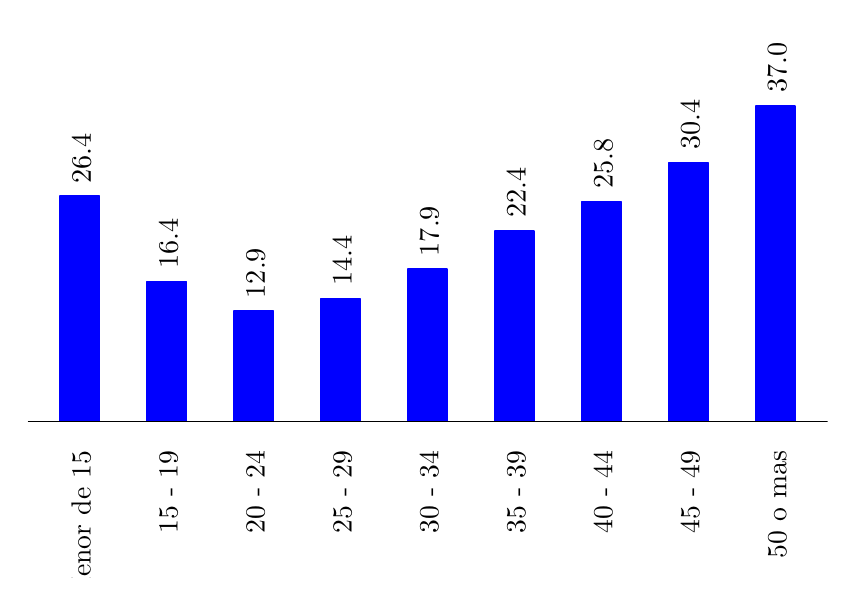
\begin{tikzpicture}[x=1pt,y=1pt]  % Created by tikzDevice version 0.10.1 on 2016-02-29 14:46:31
% !TEX encoding = UTF-8 Unicode
\definecolor{fillColor}{RGB}{255,255,255}
\path[use as bounding box,fill=fillColor,fill opacity=0.00] (0,0) rectangle (289.08,198.74);
\begin{scope}
\path[clip] (  0.00,  0.00) rectangle (289.08,198.74);

\path[] (  0.00,  0.00) rectangle (289.08,198.74);
\end{scope}
\begin{scope}
\path[clip] (  0.00,  0.00) rectangle (289.08,198.74);

\path[] (  0.00, 50.83) rectangle (289.08,176.18);

\path[] ( 18.85, 50.83) --
	( 18.85,176.18);

\path[] ( 50.27, 50.83) --
	( 50.27,176.18);

\path[] ( 81.70, 50.83) --
	( 81.70,176.18);

\path[] (113.12, 50.83) --
	(113.12,176.18);

\path[] (144.54, 50.83) --
	(144.54,176.18);

\path[] (175.96, 50.83) --
	(175.96,176.18);

\path[] (207.38, 50.83) --
	(207.38,176.18);

\path[] (238.81, 50.83) --
	(238.81,176.18);

\path[] (270.23, 50.83) --
	(270.23,176.18);
\definecolor{drawColor}{RGB}{0,0,255}
\definecolor{fillColor}{RGB}{0,0,255}

\path[draw=drawColor,line width= 0.6pt,line join=round,fill=fillColor] ( 11.78, 56.53) rectangle ( 25.92,137.81);

\path[draw=drawColor,line width= 0.6pt,line join=round,fill=fillColor] ( 43.20, 56.53) rectangle ( 57.34,106.96);

\path[draw=drawColor,line width= 0.6pt,line join=round,fill=fillColor] ( 74.63, 56.53) rectangle ( 88.77, 96.30);

\path[draw=drawColor,line width= 0.6pt,line join=round,fill=fillColor] (106.05, 56.53) rectangle (120.19,100.85);

\path[draw=drawColor,line width= 0.6pt,line join=round,fill=fillColor] (137.47, 56.53) rectangle (151.61,111.50);

\path[draw=drawColor,line width= 0.6pt,line join=round,fill=fillColor] (168.89, 56.53) rectangle (183.03,125.34);

\path[draw=drawColor,line width= 0.6pt,line join=round,fill=fillColor] (200.31, 56.53) rectangle (214.45,135.91);

\path[draw=drawColor,line width= 0.6pt,line join=round,fill=fillColor] (231.74, 56.53) rectangle (245.88,150.03);

\path[draw=drawColor,line width= 0.6pt,line join=round,fill=fillColor] (263.16, 56.53) rectangle (277.30,170.48);
\definecolor{drawColor}{RGB}{0,0,0}

\path[draw=drawColor,line width= 0.1pt,line join=round] (  0.00, 56.53) -- (289.08, 56.53);

\node[text=drawColor,rotate= 90.00,anchor=base west,inner sep=0pt, outer sep=0pt, scale=  1.02] at ( 22.82,142.51) {26.4};

\node[text=drawColor,rotate= 90.00,anchor=base west,inner sep=0pt, outer sep=0pt, scale=  1.02] at ( 54.25,111.66) {16.4};

\node[text=drawColor,rotate= 90.00,anchor=base west,inner sep=0pt, outer sep=0pt, scale=  1.02] at ( 85.67,100.99) {12.9};

\node[text=drawColor,rotate= 90.00,anchor=base west,inner sep=0pt, outer sep=0pt, scale=  1.02] at (117.09,105.54) {14.4};

\node[text=drawColor,rotate= 90.00,anchor=base west,inner sep=0pt, outer sep=0pt, scale=  1.02] at (148.51,116.19) {17.9};

\node[text=drawColor,rotate= 90.00,anchor=base west,inner sep=0pt, outer sep=0pt, scale=  1.02] at (179.93,130.03) {22.4};

\node[text=drawColor,rotate= 90.00,anchor=base west,inner sep=0pt, outer sep=0pt, scale=  1.02] at (211.35,140.60) {25.8};

\node[text=drawColor,rotate= 90.00,anchor=base west,inner sep=0pt, outer sep=0pt, scale=  1.02] at (242.78,154.72) {30.4};

\node[text=drawColor,rotate= 90.00,anchor=base west,inner sep=0pt, outer sep=0pt, scale=  1.02] at (274.20,175.17) {37.0};

\path[] (  0.00, 50.83) rectangle (289.08,176.18);
\end{scope}
\begin{scope}
\path[clip] (  0.00,  0.00) rectangle (289.08,198.74);

\path[] (  0.00, 50.83) --
	(289.08, 50.83);
\end{scope}
\begin{scope}
\path[clip] (  0.00,  0.00) rectangle (289.08,198.74);

\path[] ( 18.85, 48.08) --
	( 18.85, 50.83);

\path[] ( 50.27, 48.08) --
	( 50.27, 50.83);

\path[] ( 81.70, 48.08) --
	( 81.70, 50.83);

\path[] (113.12, 48.08) --
	(113.12, 50.83);

\path[] (144.54, 48.08) --
	(144.54, 50.83);

\path[] (175.96, 48.08) --
	(175.96, 50.83);

\path[] (207.38, 48.08) --
	(207.38, 50.83);

\path[] (238.81, 48.08) --
	(238.81, 50.83);

\path[] (270.23, 48.08) --
	(270.23, 50.83);
\end{scope}
\begin{scope}
\path[clip] (  0.00,  0.00) rectangle (289.08,198.74);
\definecolor{drawColor}{RGB}{0,0,0}

\node[text=drawColor,rotate= 90.00,anchor=base east,inner sep=0pt, outer sep=0pt, scale=  1.00] at ( 22.76, 45.88) {Menor de 15};

\node[text=drawColor,rotate= 90.00,anchor=base east,inner sep=0pt, outer sep=0pt, scale=  1.00] at ( 54.18, 45.88) {15 - 19};

\node[text=drawColor,rotate= 90.00,anchor=base east,inner sep=0pt, outer sep=0pt, scale=  1.00] at ( 85.60, 45.88) {20 - 24};

\node[text=drawColor,rotate= 90.00,anchor=base east,inner sep=0pt, outer sep=0pt, scale=  1.00] at (117.03, 45.88) {25 - 29};

\node[text=drawColor,rotate= 90.00,anchor=base east,inner sep=0pt, outer sep=0pt, scale=  1.00] at (148.45, 45.88) {30 - 34};

\node[text=drawColor,rotate= 90.00,anchor=base east,inner sep=0pt, outer sep=0pt, scale=  1.00] at (179.87, 45.88) {35 - 39};

\node[text=drawColor,rotate= 90.00,anchor=base east,inner sep=0pt, outer sep=0pt, scale=  1.00] at (211.29, 45.88) {40 - 44};

\node[text=drawColor,rotate= 90.00,anchor=base east,inner sep=0pt, outer sep=0pt, scale=  1.00] at (242.71, 45.88) {45 - 49};

\node[text=drawColor,rotate= 90.00,anchor=base east,inner sep=0pt, outer sep=0pt, scale=  1.00] at (274.14, 45.88) {50 o mas};
\end{scope}
  \end{tikzpicture}}{Instituto Nacional de Estadística, de las Estadísticas Vitales 2014}
